\chapter{CISLUNAR DEPARTURE ORBIT COMPARISON}

The two approaches introduced in the previous chapter for designing end-to-end transfers from the
cislunar region to Mars generate families of transfers from various departure unstable periodic
orbits in Earth-Moon CR3BP families. For given departure orbits, the transfers that stage
in an intermediate Sun-Earth halo orbit are compared to the transfers with direct departures from
the Sun-Earth system to determine any potential benefits of a staging orbit. A cost function is
introduced to aid in the selection of desirable transfers in each transfer group. Then the selected
transfers are compared across the various cislunar departure orbits to analyze the departure
characteristics across orbit families and energy levels. Finally, the total maneuver $\Delta v$
and TOF costs of the transfer strategies developed in this investigation are compared to existing
literature and methodologies to demonstrate that this approach reduces the maneuver costs for a
Mars mission.

\section{Comparing Transfers via Sun-Earth Staging Orbits to Direct Transfers}\label{sec:StagingComparison}
Just like the example tradespace provided in \cref{sec:Transfers} with \cref{fig:tradespace}, for a
given cislunar departure orbit, the direct transfers are compared to the staging orbit ones. The
tradespaces for all of the cislunar departure orbits utilized in this investigation are provided in
\cref{chap:Tradespaces}, along with figures illustrating the departure orbits themselves, but some
are introduced in this section to facilitate the comparison. In general, for the scenarios examined
in this investigation, transfers with lower times-of-flight tend to have higher maneuver costs and
vice versa. As demonstrated in the example of \cref{fig:tradespace}, the transfer points lie mostly
in the upper-left and bottom-right sections of the tradespace. In all of the tradespaces computed
in this investigation, the blue points representing the direct transfers mostly lie to the left of
the red staging orbit transfers but well above the modified Hohmann transfer baseline,
corresponding to direct transfers with lower TOF but much higher $\Delta v$ compared to the staging
orbit transfers. However, there are often some transfers in the tradespace where the $\Delta v$
lies below the baseline of the modified Hohmann transfer and even below those of the staging orbit
transfers. The tradeoff between time-of-flight and maneuver cost highlights the importance of
mission-specific priorities when selecting a transfer strategy.


\subsection{A Simple Cost Function}
In the example of \cref{fig:tradespace}, the transfer family that directly departs the system
contains both the minimum-TOF and minimum-$\Delta v$ solutions. In the provided case, the
minimum-$\Delta v$ solution of the direct transfers has a lower TOF than most of the staging orbit
transfers. However, this is not always the case, as demonstrated by \cref{fig:lowDeltav}. Here,
while the direct transfers still have a lower TOF, the staging orbit transfer family reaches a
lower $\Delta v$. As a result, often a transfer selection needs to be made balancing TOF and
maneuver cost. A cost function helps select desirable transfers that balance the two parameters.

\begin{figure}[H]
    \centering
    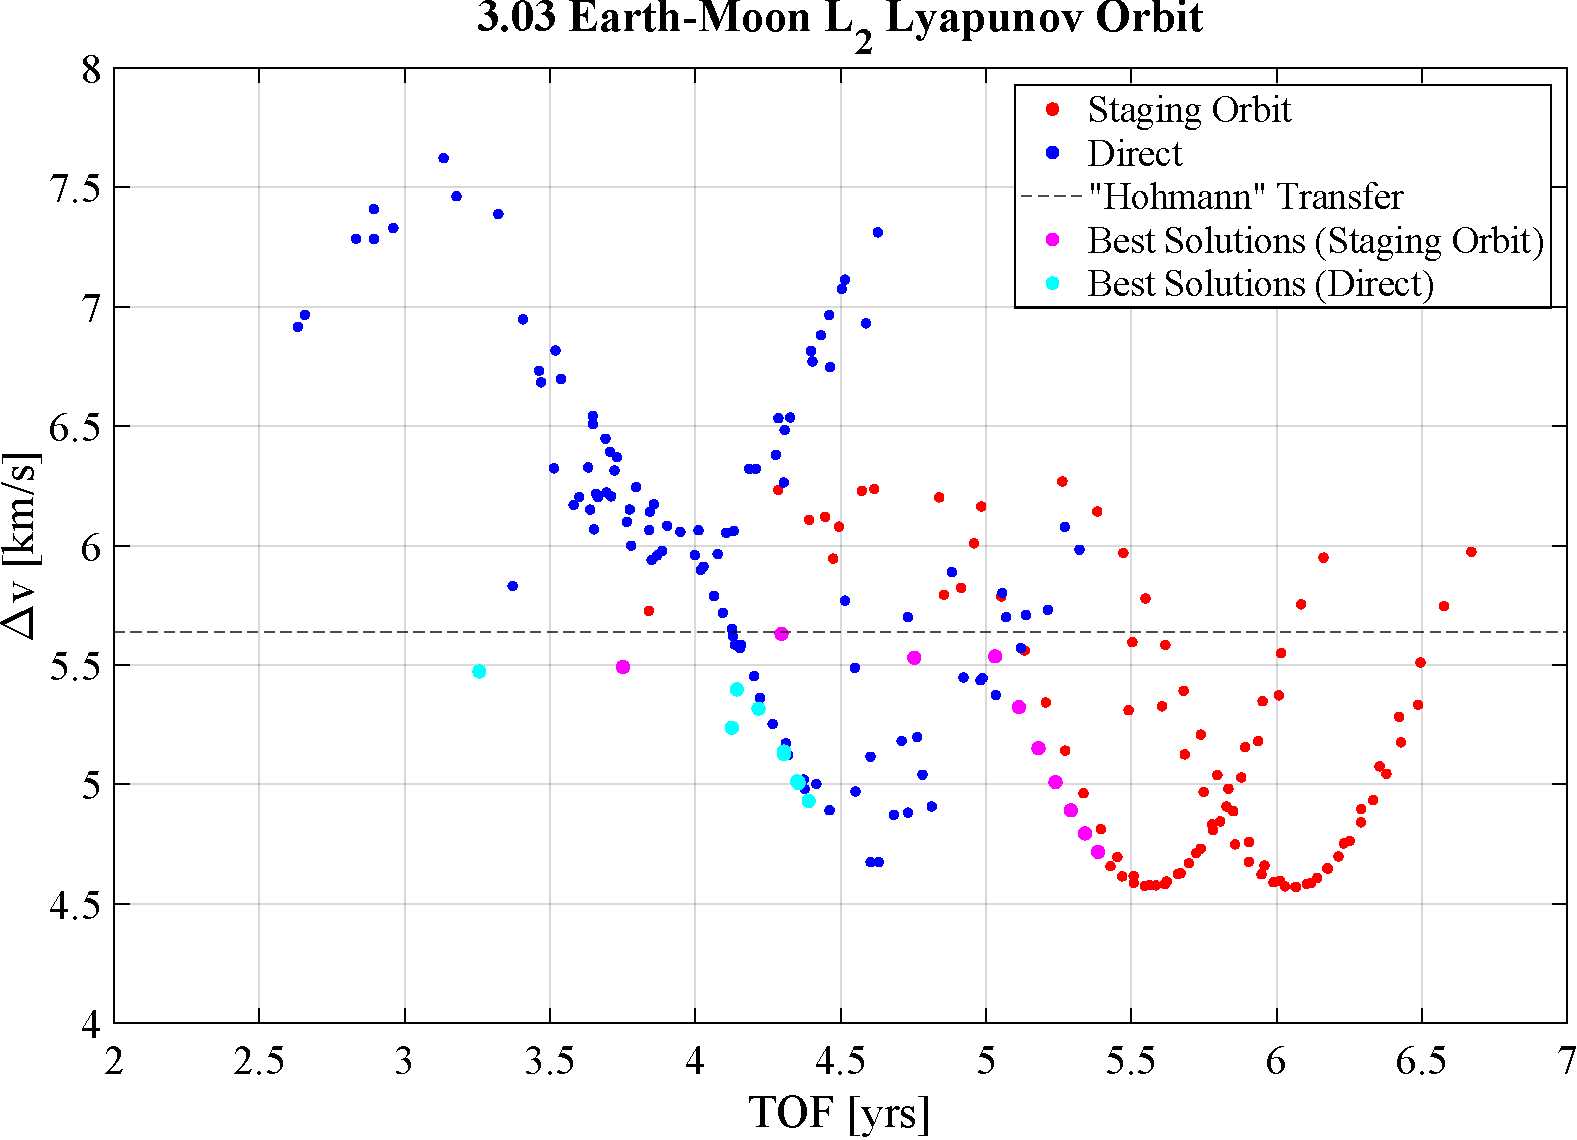
\includegraphics[width=0.75\textwidth]{figures/TradeSpace_L2Lyapunov_3_03.pdf}
    \caption{Transfer tradespace departing from an Earth-Moon $L_{2}$ Lyapunov orbit ($JC=3.03$).}
    \label{fig:lowDeltav}
\end{figure}

If total TOF and total maneuver $\Delta v$ are considered to have units of years and km/s,
respectively, then the values have similar orders of magnitude for the computed transfers.
Consequently, an appropriate cost function places weights on the two parameters according to the
desired transfer characteristics for a given mission:
\begin{equation}
    J=\alpha TOF+\beta\Delta v,
    \label{eq:costfunction}
\end{equation}
where $J$ is the cost function value and $\alpha$ and $\beta$ are design variables for adjusting
the cost function. $\alpha$ and $\beta$ can be adjusted to place higher priority on TOF or
$\Delta v$, depending on the particular application. This investigation utilizes values of
$\alpha=5$ and $\beta=2$ as a representative cost function to prioritize lowering the TOF while
still looking for decreased maneuver costs. The cost function is applied to transfers in the
tradespace that are below the modified Hohmann transfer $\Delta v$ baseline, and the ten transfers
that have the lowest $J$-value from each transfer category are determined to be the lowest-cost
transfers for the selected application. In \cref{fig:lowDeltav}, there are cyan points for the
direct transfers and magenta ones for the staging orbit transfers. The cost function provides a
systematic approach to identify transfers that balance time-of-flight and maneuver costs, ensuring
that the selection aligns with mission priorities and operational constraints.

\subsection{Comparing Lowest-Cost Solutions between Transfer Types}
Comparing the lowest-cost solutions highlights the differences between direct transfers and staging
orbit transfers, with direct options generally achieving shorter times-of-flight at slightly higher
or comparable maneuver costs. In \cref{fig:lowDeltav}, among the lowest-cost solutions selected
with the cost function, the direct options have a lower average TOF than the staging orbit ones,
$4.04$ and $4.94$ years, respectively, while the transfers with staging orbits achieve a slightly
lower average $\Delta v$ cost, $5.207$ km/s compared to $5.238$. The earlier example from
\cref{fig:tradespace}, now including the lowest-cost solutions from the cost function in
\cref{fig:costTradespace}, produces similar results. In contrast, the direct options in
\cref{fig:lowBoth} have both lower times-of-flight and maneuver costs when compared to the staging
orbit transfers, $4.33$ years and $4.869$ km/s average for direct transfers versus $4.82$ years and
$5.148$ km/s for those with a staging orbit. In all of the tradespaces computed in this
investigation, the lowest-cost direct solutions perform better than the lowest-cost staging orbit
transfers with regards to TOF. While the lowest-cost staging orbit solutions often have slightly
lower $\Delta v$ costs on average, the significantly longer times-of-flight outweigh those
benefits, and there are still many cases where the direct options require lower maneuver costs.

\begin{figure}[H]
    \centering
    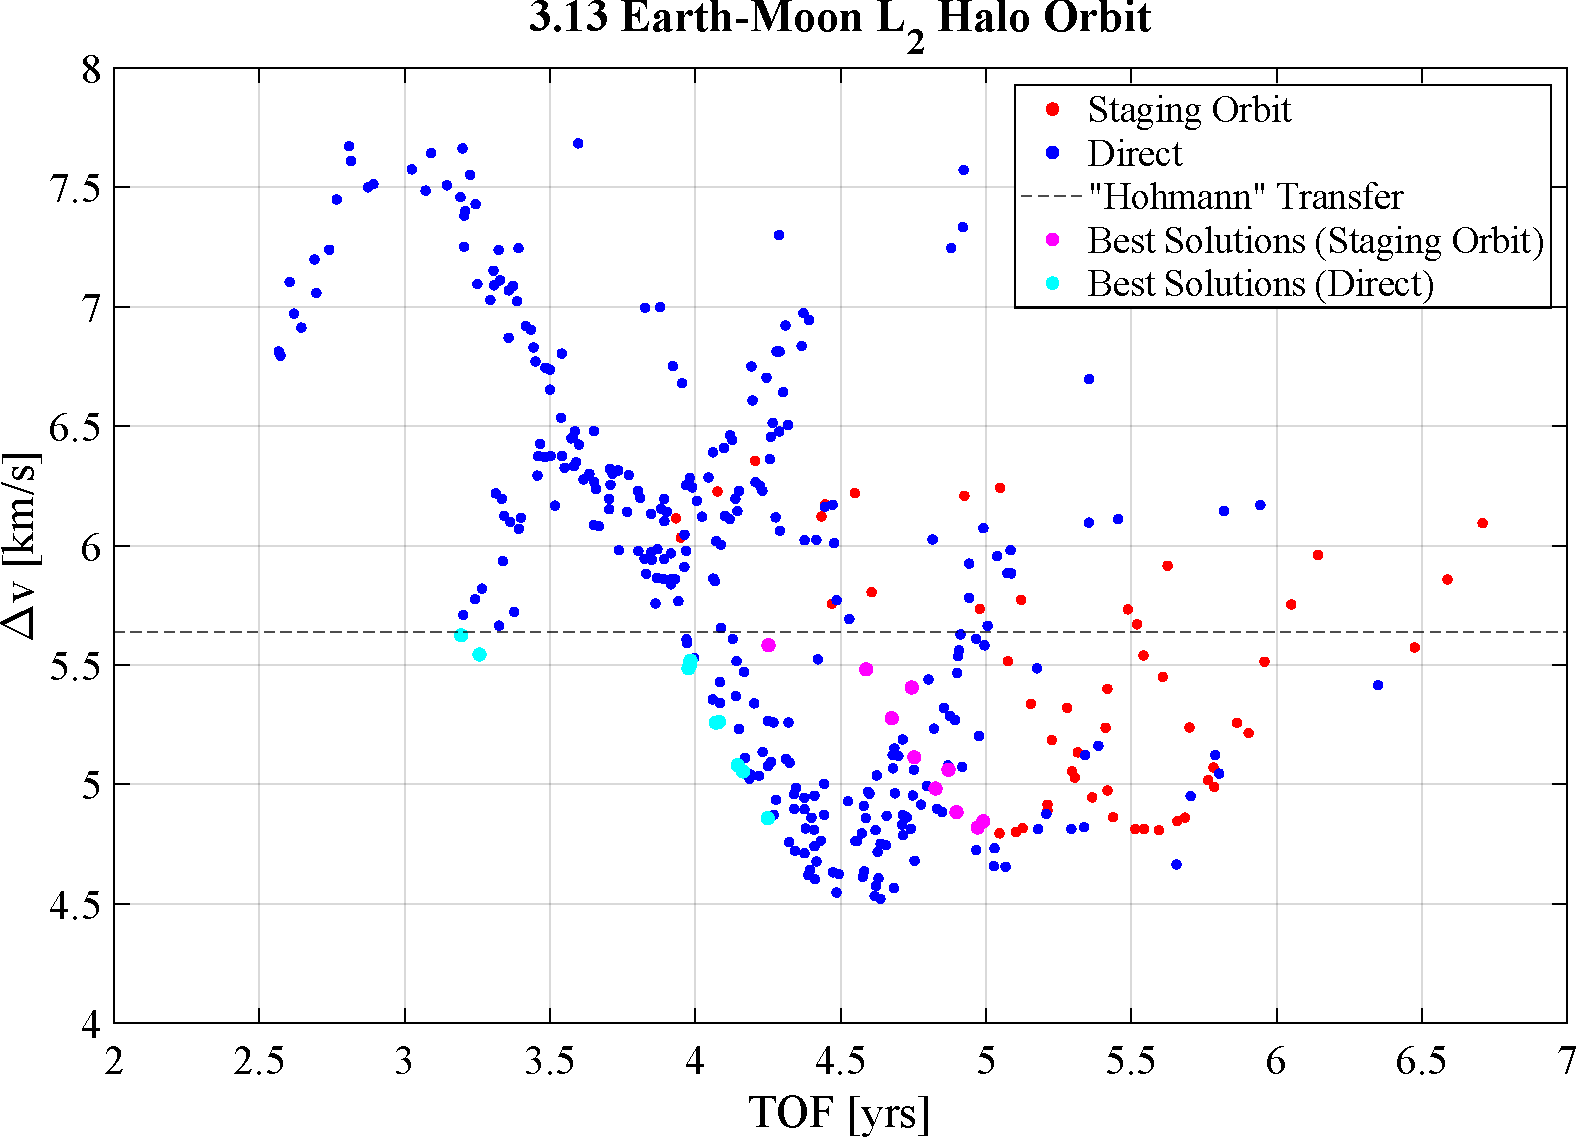
\includegraphics[width=0.75\textwidth]{figures/TradeSpace_L2Halo_3_13.pdf}
    \caption{Transfer tradespace departing from an Earth-Moon $L_{2}$ northern halo orbit ($JC=3.13$).}
    \label{fig:costTradespace}
\end{figure}

One downside to the direct departure method is that it relies on the spread and rapid departure of
the Earth-Moon unstable manifolds arcs. A major contributing factor is the proximity of the
cislunar orbit to the Moon or Earth. If manifold arcs crash into one of the primaries or get
captured by their gravitational effects, it delays the departure of the arcs from the system and
also impacts their distribution in position space, leading to fewer available transfers. The
stability of the orbit also plays a role in affecting the departure time since orbits with higher
instability have manifolds that depart the orbit vicinity faster. When there are fewer departure
arcs available, it leads to fewer successful end-to-end transfers with direct departures,
demonstrated in \cref{fig:fewDirect}. Note that there is a significantly decreased number of
available direct solutions and that the ones that do exist no longer follow a familial pattern as
in the previous examples. Since the staging orbit transfers only require one manifold arc to
interface with the Sun-Earth orbit stable manifold, there is still a full range of staging orbit
transfers available. However, the lowest-cost direct solutions still outperform the staging orbit
ones here.

\begin{figure}[H]
    \centering
    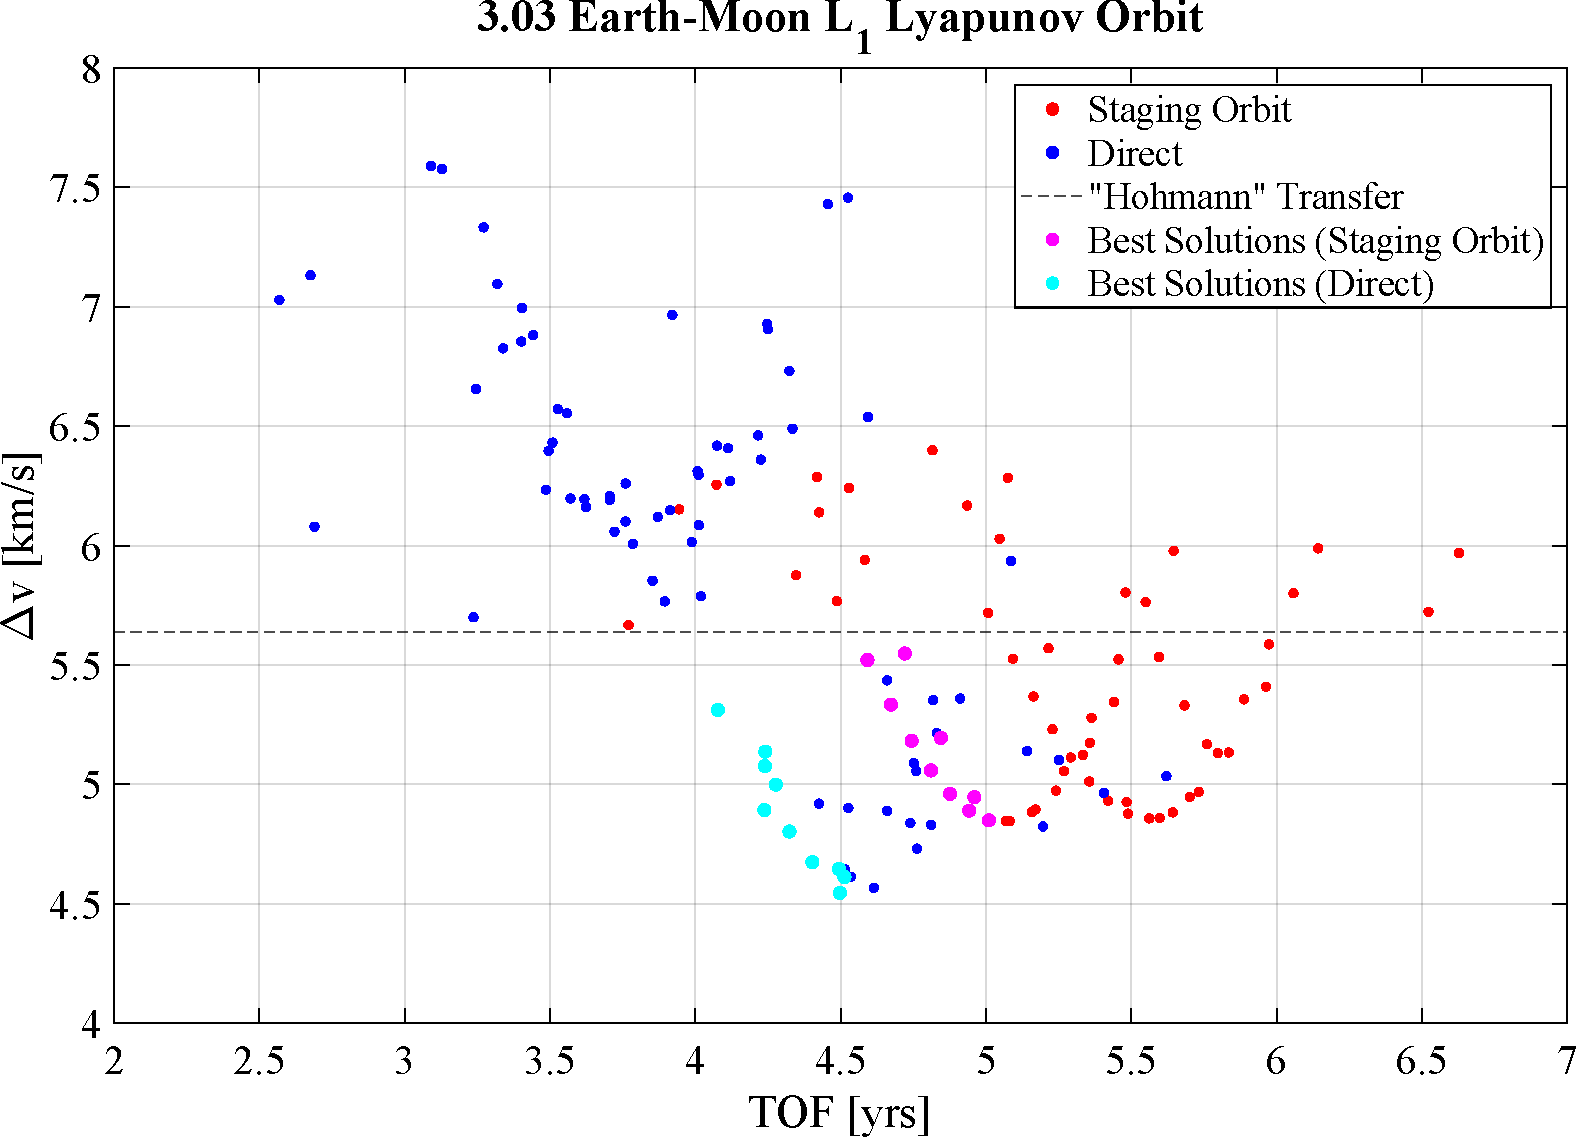
\includegraphics[width=0.75\textwidth]{figures/TradeSpace_L1Lyapunov_3_03.pdf}
    \caption{Transfer tradespace departing from an Earth-Moon $L_{1}$ Lyapunov orbit ($JC=3.03$).}
    \label{fig:lowBoth}
\end{figure}

The results of this investigation and the provided observations demonstrate that the methodology
developed to construct end-to-end cislunar-to-Mars transfers that directly depart the Sun-Earth
system performs better overall than the strategy that incorporates an intermediate Sun-Earth halo
staging orbit. The lowest-cost solutions that directly depart the cislunar orbits utilized in this
investigation always have a faster average TOF than the lowest-cost staging orbit transfers. While
the direct options only sometimes have a lower $\Delta v$ maneuver cost than the staging orbit
ones, the decrease in TOF is significant enough to outweigh the potential slight increases in
maneuver cost. The findings highlight the efficiency and practicality of direct transfer options
for mission planning, particularly when the minimization of TOF is a critical mission objective.

\begin{figure}[H]
    \centering
    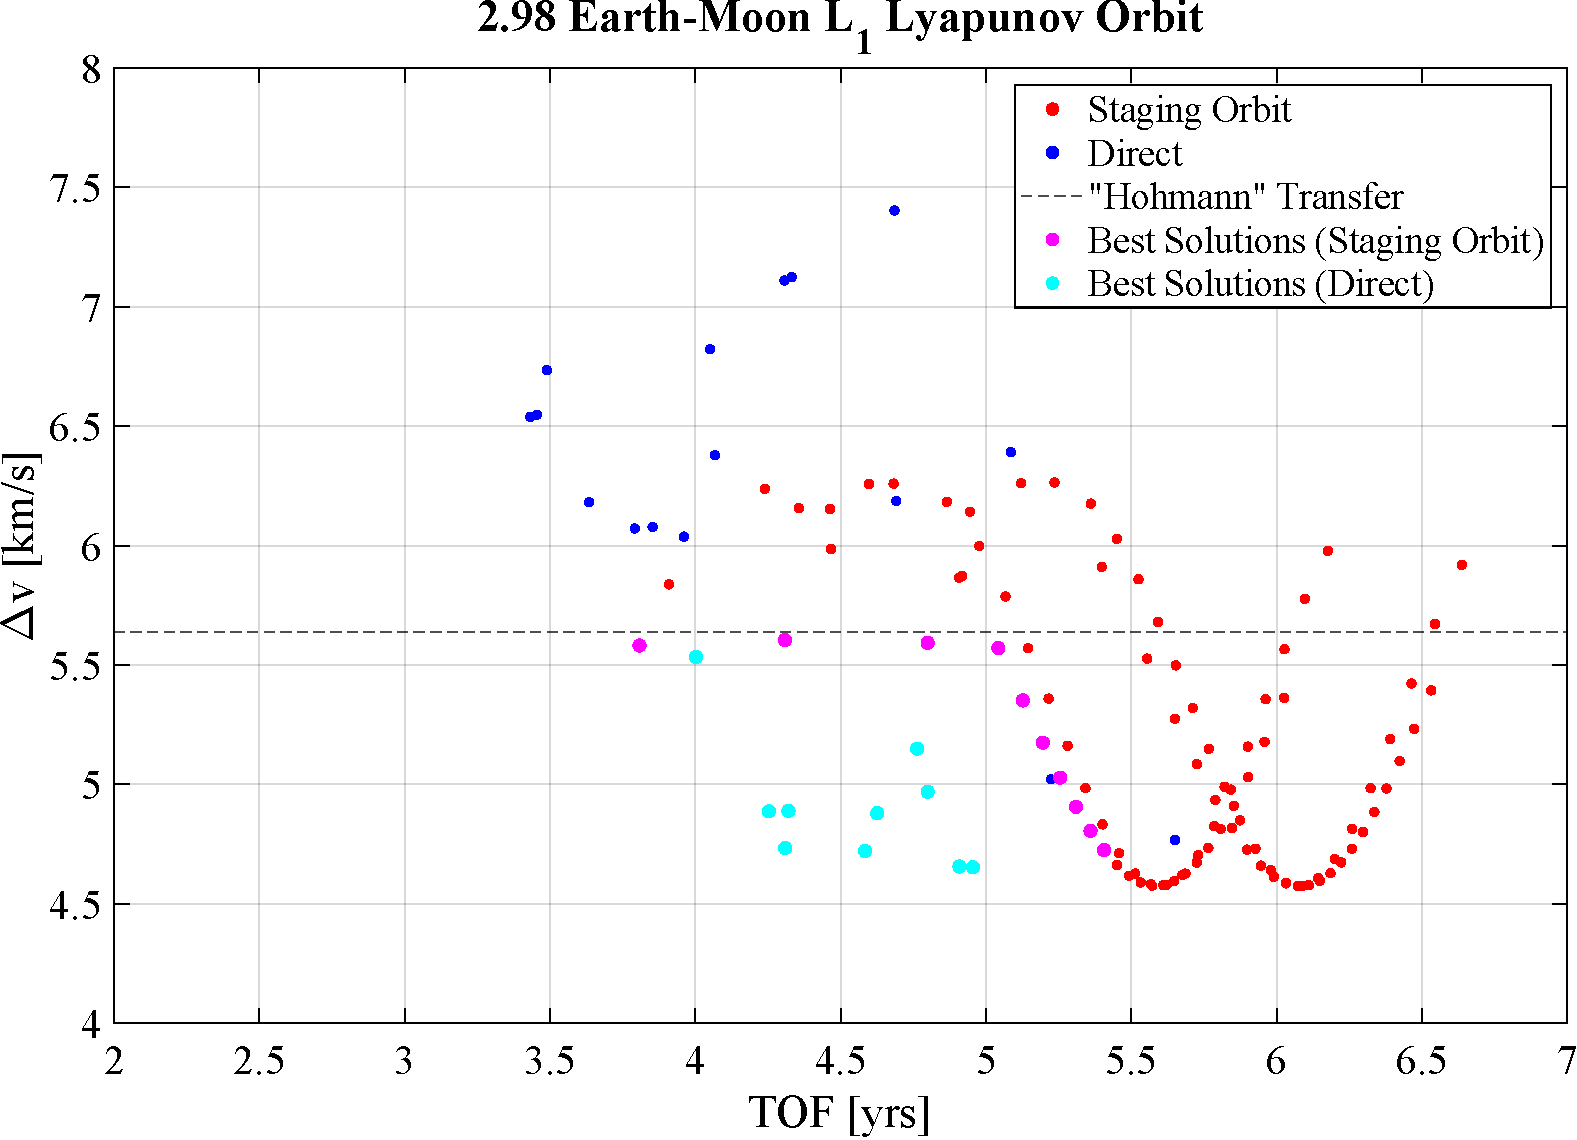
\includegraphics[width=0.75\textwidth]{figures/TradeSpace_L1Lyapunov_2_98.pdf}
    \caption{Transfer tradespace departing from an Earth-Moon $L_{1}$ Lyapunov orbit ($JC=2.98$).}
    \label{fig:fewDirect}
\end{figure}

\section{Comparing Cislunar Departure Families}
In this investigation, unstable periodic orbits in the Earth-Moon CR3BP are considered as potential
departure orbits for deep space transfers. Several orbit families with unstable members are
introduced in Section 3.2 and from these families, unstable orbits between Jacobi constants of
$2.98$ and $3.13$ are analyzed to determine their feasibility for these transfers. This range was
chosen since the upper energy bound of $2.98$ is slightly above the energy level of the $L_{4}$ and
$L_{5}$ Lagrange points, while the lower bound includes a large number of the unstable libration
orbits\cite{Zimovan:2017}. Note that not all of the included families have unstable orbits at these
energy levels. Additionally, in some instances, even though the orbits existed, their stability,
energy, or location prevented their unstable invariant manifolds from interfacing with the stable
manifolds of the staging orbit or departing the system promptly. Several other periodic orbit
families were also investigated, including $L_{4}$ and $L_{5}$ long-period orbits and some unstable
resonant orbit families. However, invariant manifolds from orbits in these families also took too
long to depart the system for this investigation.

For the feasible departure orbits, the cost function described previously is used to determine the
most desirable end-to-end transfers in the orbit's tradespace, and then the average total
maneuver $\Delta v$ and TOF costs are compared between the various departure orbits in this
investigation. While no one orbit or family of orbits provides the lowest-cost transfers across the
different energy levels, some trends can be extracted from the results to inform cislunar departure
orbit selection for these types of missions.

\subsection{Contributing Factors for Lower Total Maneuver Costs}
Of the two maneuvers, or three if using a staging orbit, in the end-to-end transfer, the largest is
the final burn that includes the inclination change between the Sun-Earth and Sun-Mars planes.
Plane change maneuvers are most efficient at a conic orbit's apoapsis, so this maneuver $\Delta v$
is lower when the MMAT bridge conic true anomaly at the intersection of the conic sections,
$\theta_{b_{int}}$, is near $\ang{180}$. This also requires that the departure and bridge conics
are oriented such that their apoapses are near the line of nodes since the inclination change must
occur at either the ascending or descending node. The conic intersection location is a function of
the relative orientations of the departure and arrival conics, which are dependent on the phasing
of the departure from and arrival at the two planetary systems. 

As mentioned, the cost function identifies the transfers with the lowest cost, considering both the
maneuver cost and TOF. Therefore, among the ten lowest-cost transfers in a tradespace, there will
be ones with lower total $\Delta v$ and and ones with a lower TOF.
\cref{fig:stagedMinDvEM}-\cref{fig:stagedMinDvMMAT} show an example staging orbit low-$\Delta v$
case departing from a northern $L_{1}$ halo orbit, with a total maneuver cost of $4.781$ km/s and
TOF of $5.21$ years. Likewise, \cref{fig:directMinDvE} and \cref{fig:directMinDvMMAT} show a direct
example departing from an $L_{1}$ Lyapunov orbit, with a total maneuver cost of $4.55$ km/s and TOF
of $4.49$ years. In both MMAT figures, \cref{fig:stagedMinDvMMAT} and \cref{fig:directMinDvMMAT},
the two maneuvers occur approximately $\ang{180}$ apart from each other, and since the first burn
is constrained to be at the periapsis of the bridge conic, the second burn is near apoapsis. Note
that in the transfer example with direct departure, the manifold arc chosen departs on the $L_{2}$
side of the Sun-Earth system. This is consistent for lower-$\Delta v$ direct transfers across all
the departure orbits analyzed in this investigation.

\begin{figure}[!htb]
    \centering
    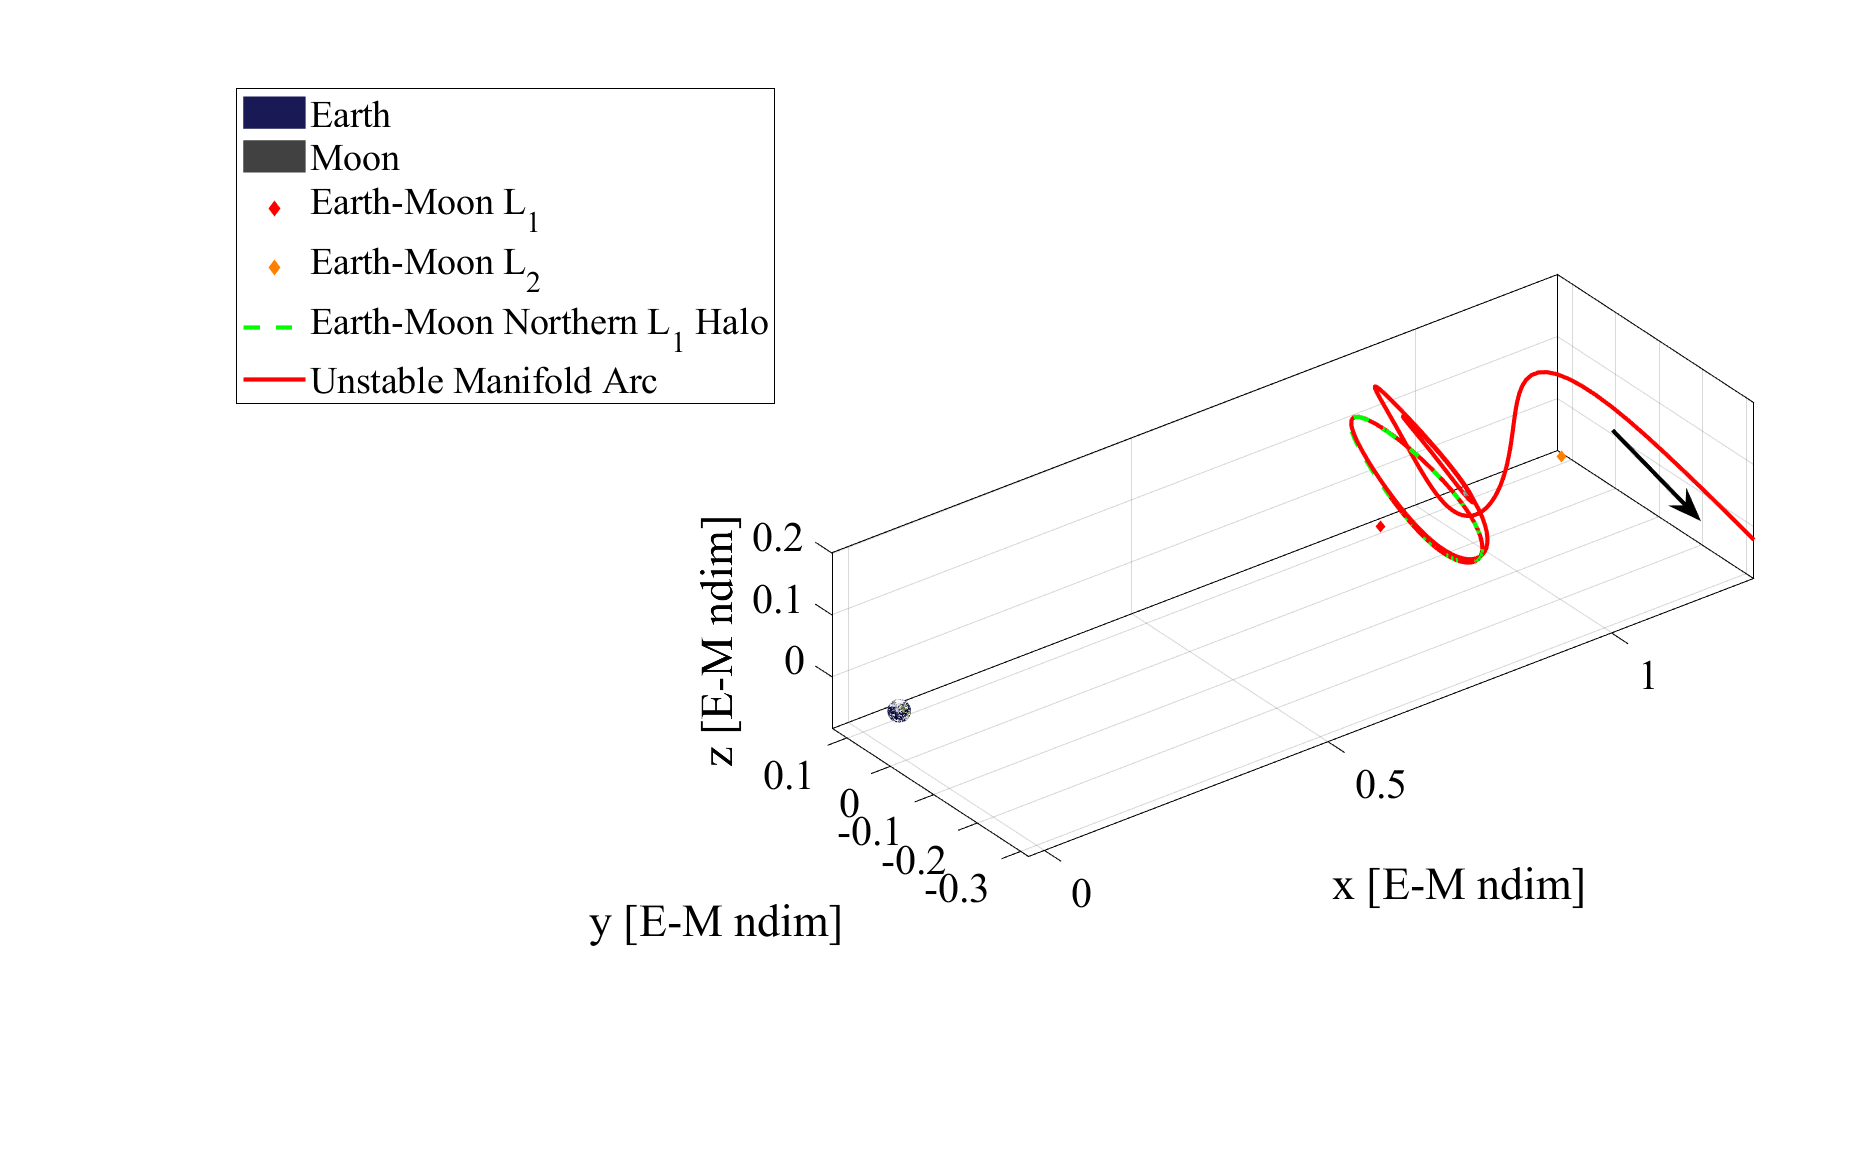
\includegraphics[width=0.9\textwidth]{figures/StagedMinDvEM.pdf}
    \caption{Northern $L_{1}$ halo orbit ($JC=3.03$) departure manifold arc in the Earth-Moon barycentric rotating frame for a low-$\Delta v$ case.}
    \label{fig:stagedMinDvEM}
\end{figure}

\begin{figure}[!htb]
    \centering
    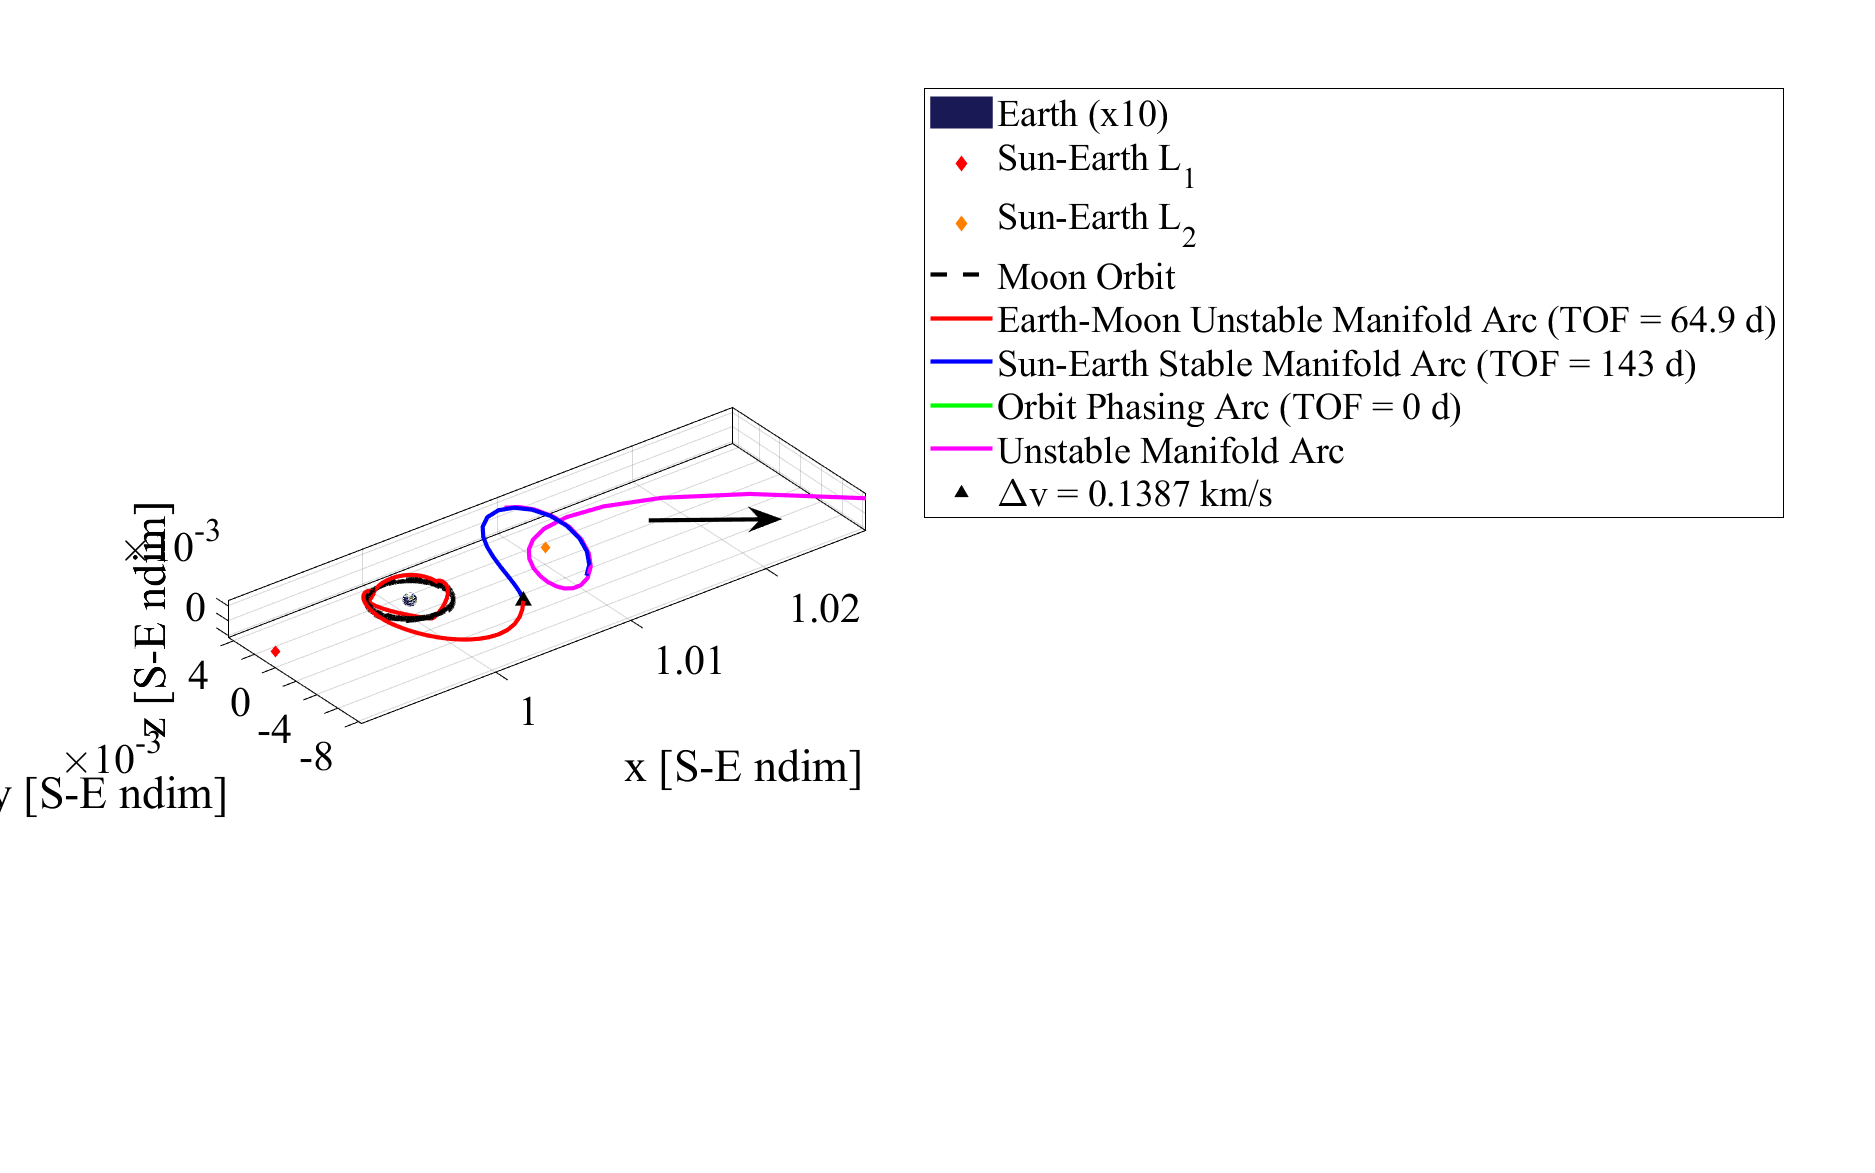
\includegraphics[width=0.9\textwidth]{figures/StagedMinDvSE.pdf}
    \caption{Departure CR3BP arc with northern $L_{2}$ halo staging orbit ($JC=3.000808$) in the Sun-Earth barycentric rotating frame for a low-$\Delta v$ case.}
    \label{fig:stagedMinDvSE}
\end{figure}

\begin{figure}[!htb]
    \centering
    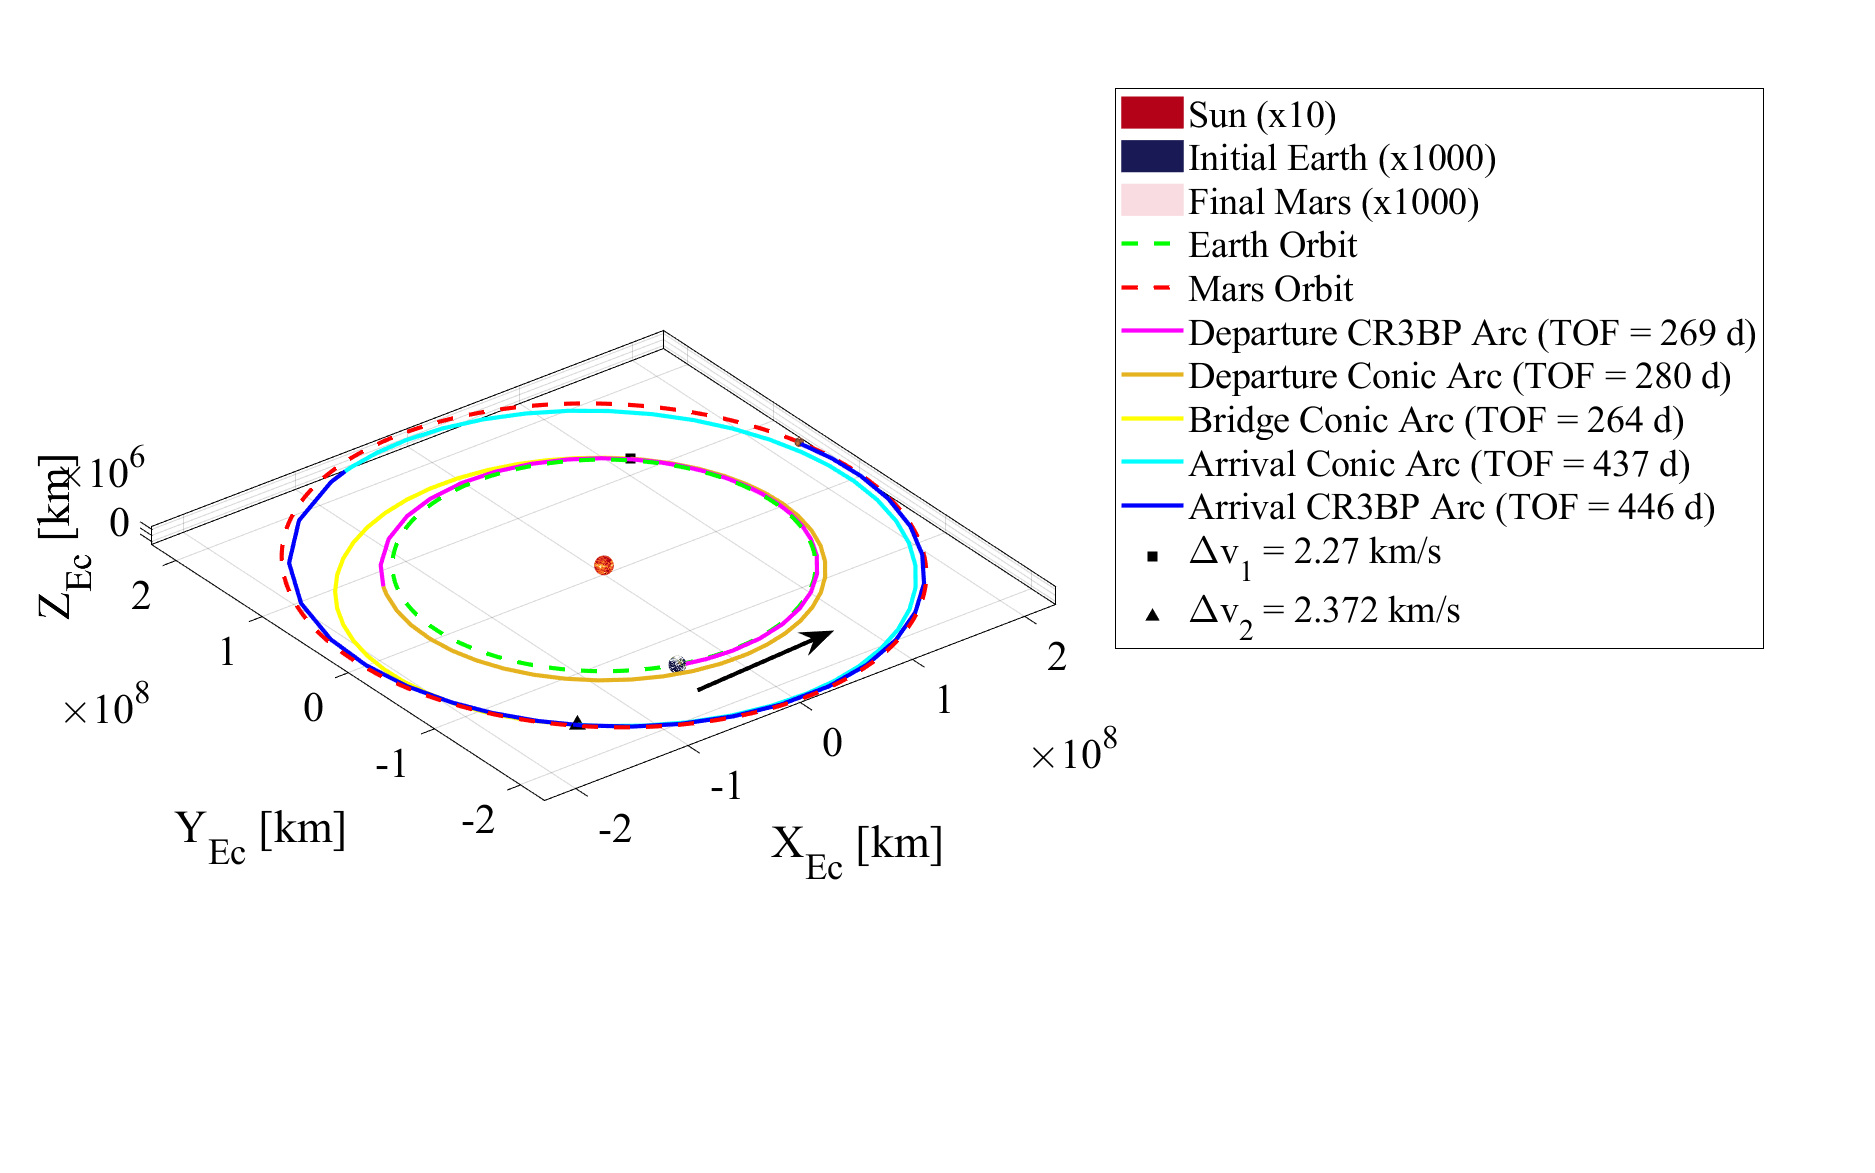
\includegraphics[width=0.9\textwidth]{figures/StagedMinDvMMAT.pdf}
    \caption{MMAT in the Sun-centered Ecliptic J2000 frame for a staging orbit low-$\Delta v$ case.}
    \label{fig:stagedMinDvMMAT}
\end{figure}

\begin{figure}[!htb]
    \begin{subfigure}[h]{0.495\linewidth}
        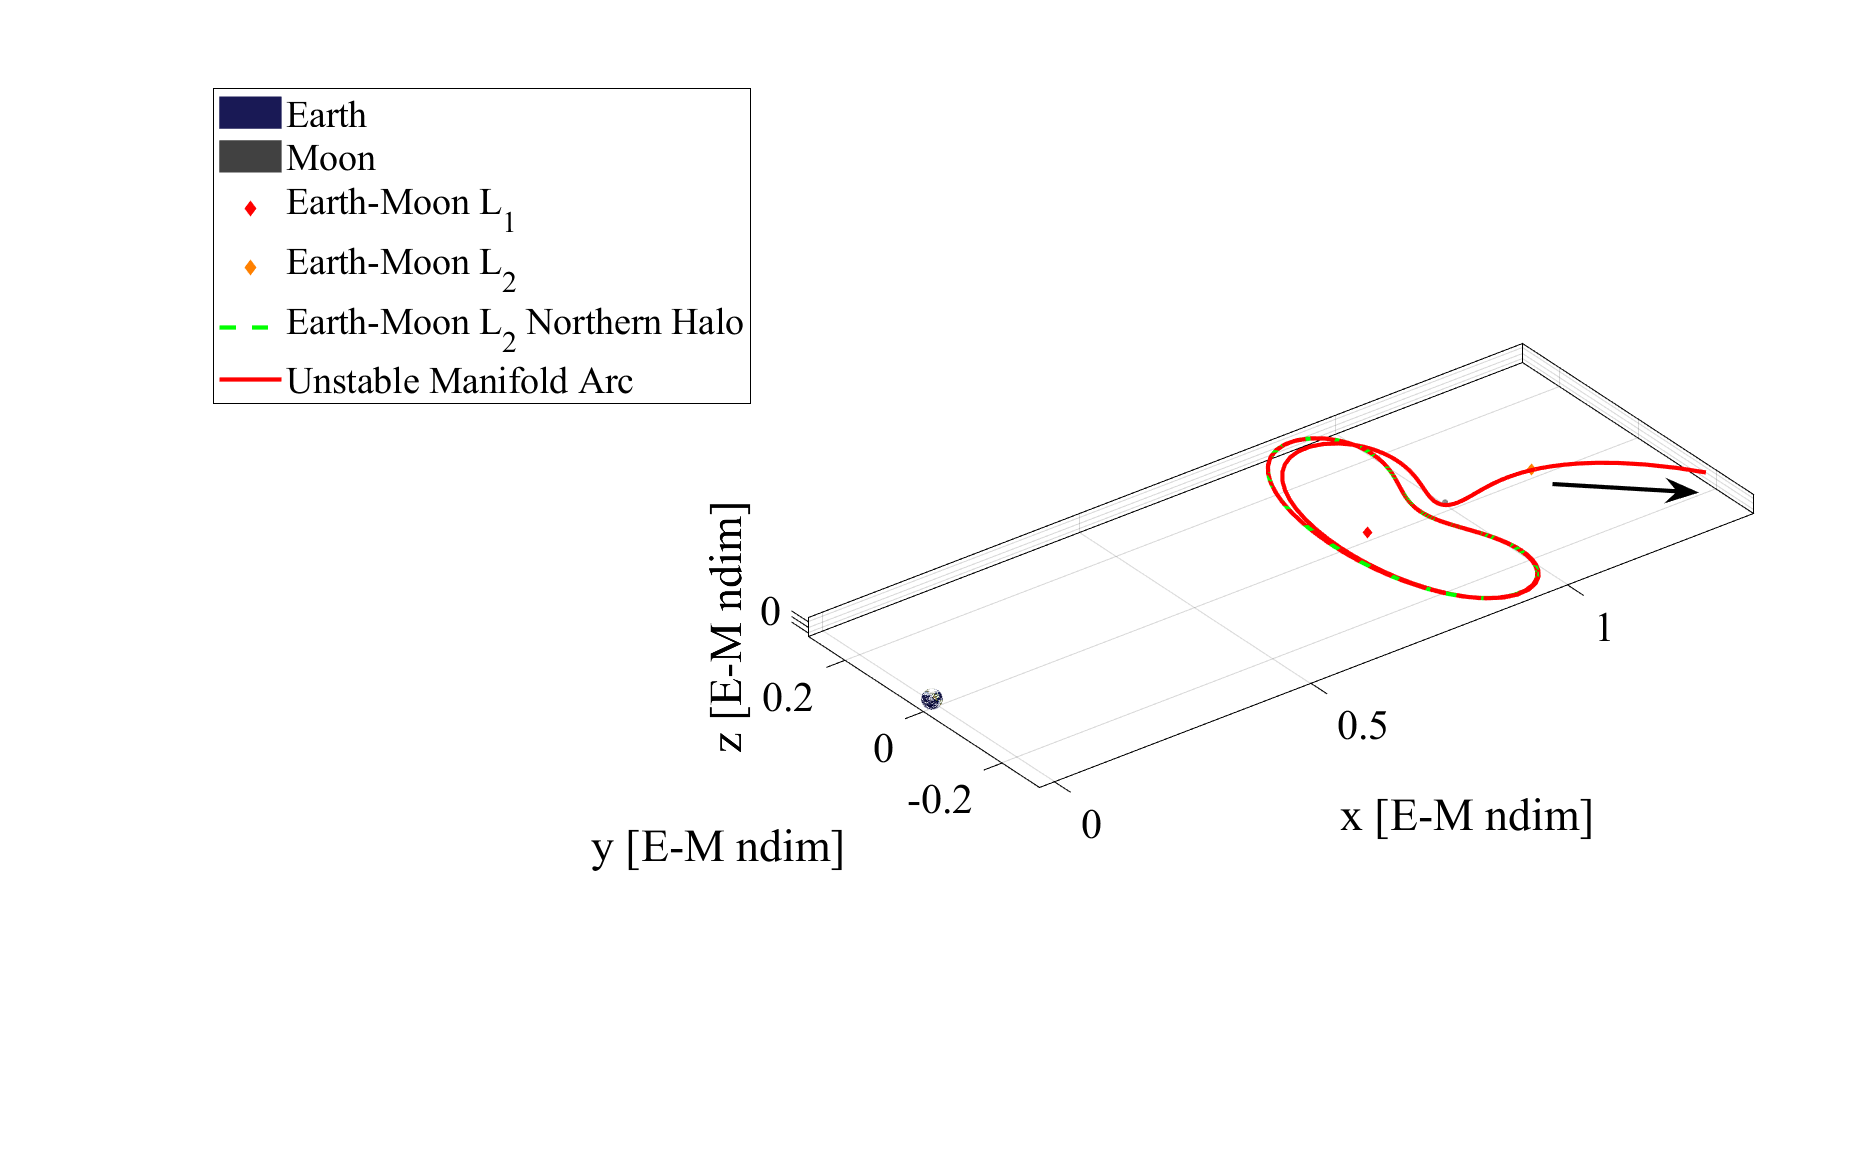
\includegraphics[width=\textwidth]{figures/DirectMinDvEM.pdf}
        \caption{Earth-Moon barycentric rotating frame.}
    \end{subfigure}
    \hfill
    \begin{subfigure}[h]{0.495\linewidth}
        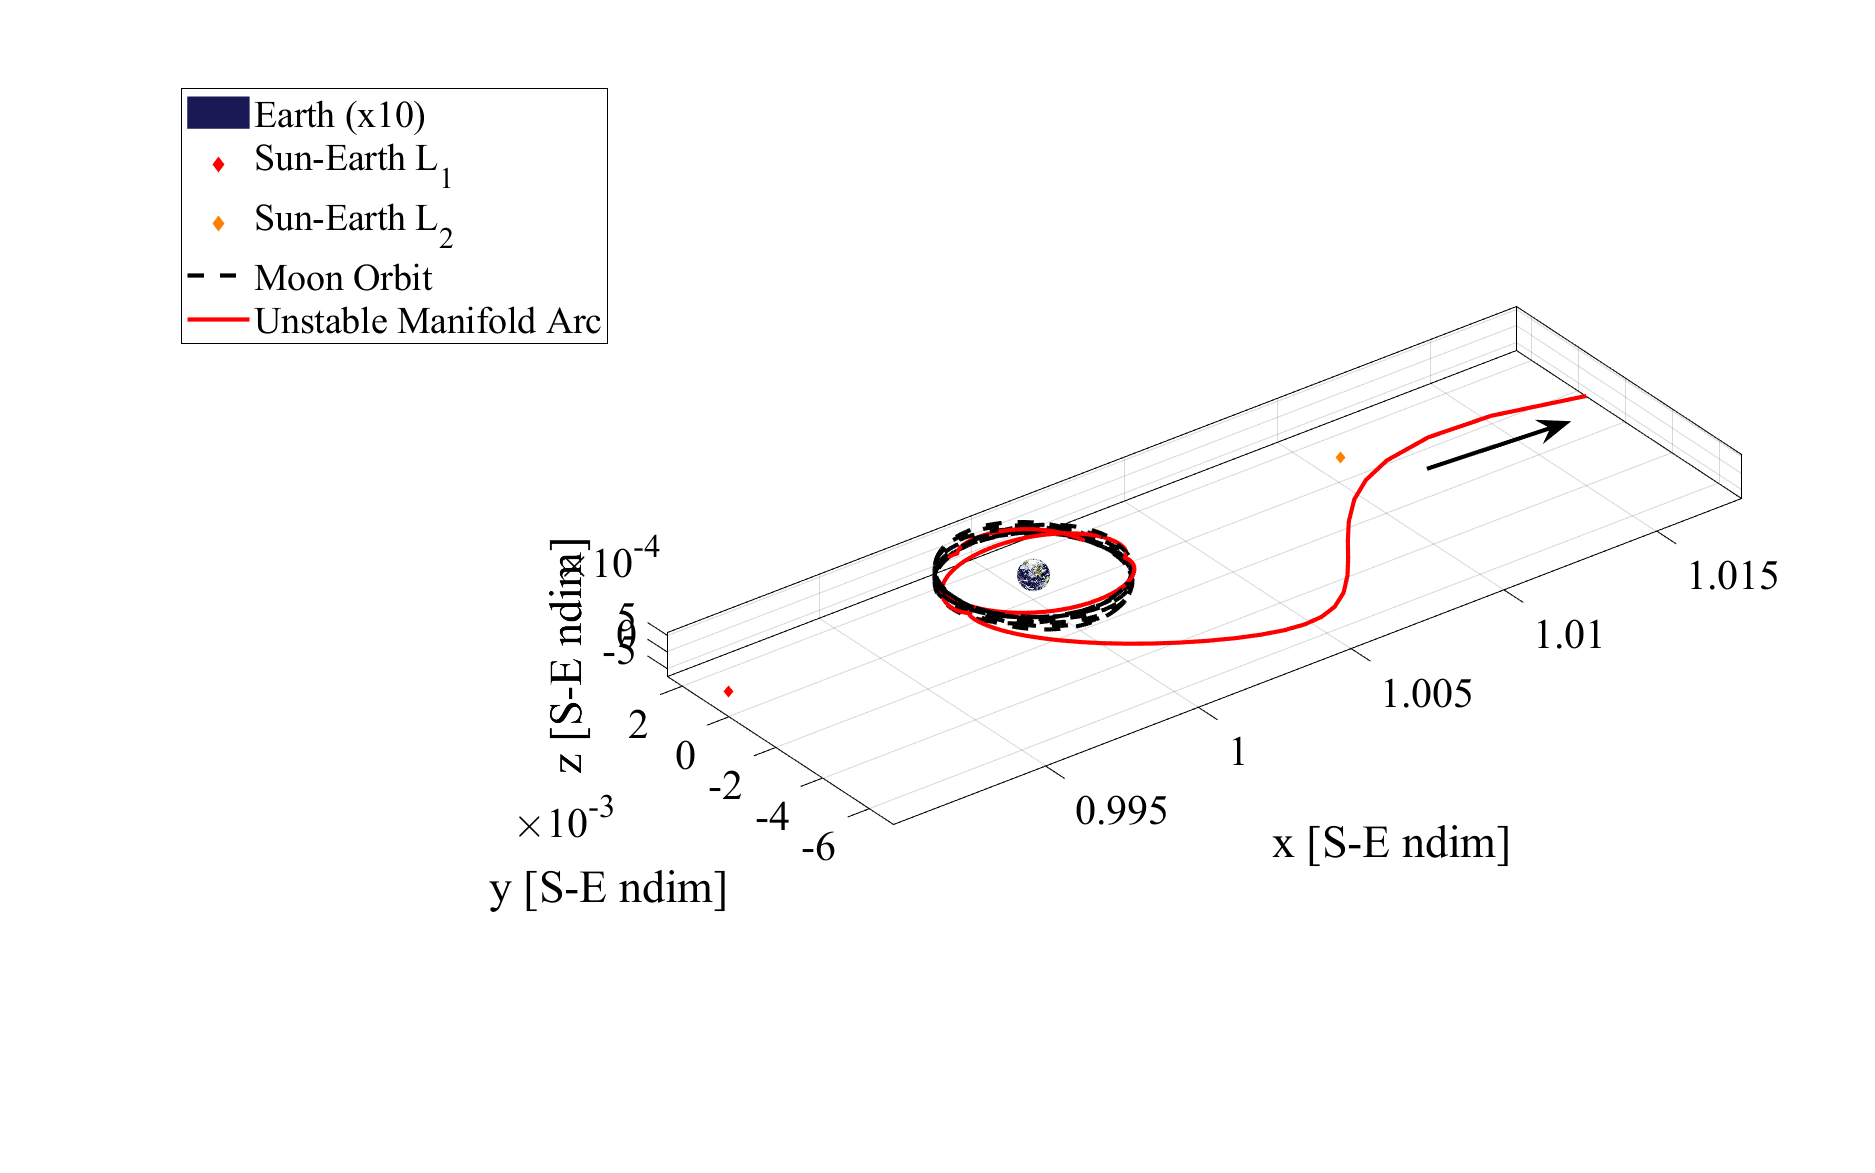
\includegraphics[width=\textwidth]{figures/DirectMinDvSE.pdf}
        \caption{Sun-Earth barycentric rotating frame.}
    \end{subfigure}
    \caption{$L_{1}$ Lyapunov orbit ($JC=3.0$) departure CR3BP arc for a low-$\Delta v$ case.}
    \label{fig:directMinDvE}
\end{figure}

\begin{figure}[!htb]
    \centering
    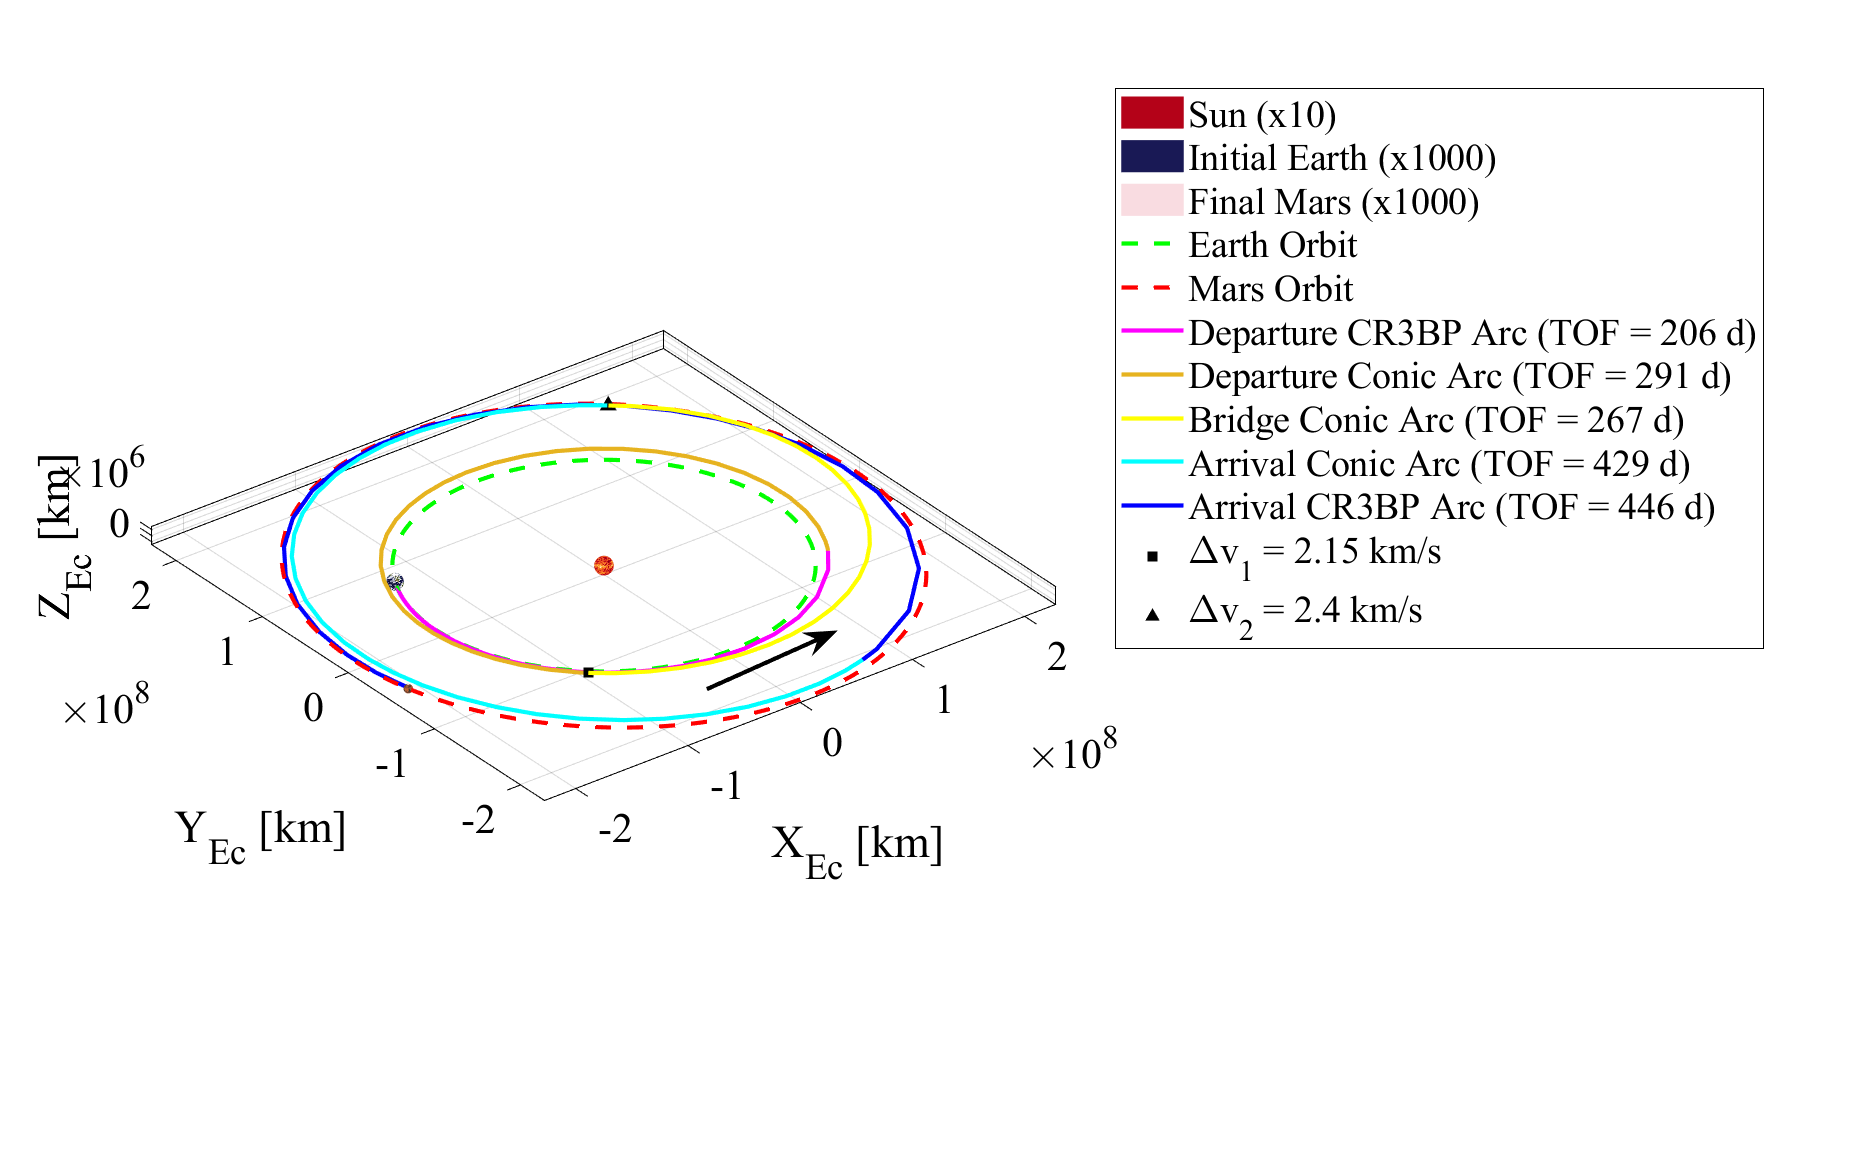
\includegraphics[width=0.9\textwidth]{figures/DirectMinDvMMAT.pdf}
    \caption{MMAT in the Sun-centered Ecliptic J2000 frame for a direct low-$\Delta v$ case.}
    \label{fig:directMinDvMMAT}
\end{figure}

Beyond the relative orientation between the two MMAT maneuvers, the energy gap between the
departure and arrival arcs (and thereby the Sun-Earth and Sun-Mars CR3BP arcs, respectively) also
contributes to the total $\Delta v$. A larger difference requires a higher-cost maneuver to change
the Keplerian conic energy from the departure arc to that of the arrival arc; these energies are
determined by the manifold arcs chosen and the phasing of the two planetary systems. This
highlights the importance of families of transfer solutions. Since several interdependent factors
affect the total maneuver cost, it is necessary to search through the results across families of
solutions to find low-$\Delta v$ solution basins.

\subsection{Contributing Factors for Lower Total Times-of-Flight}
While $\Delta v$ is primarily dependent on the final MMAT maneuver location, the biggest factor
affecting time-of-flight is the relative orientation of the departure and arrival conic arcs. Since
these are dependent on their respective CR3BP manifold arcs, the phasing of the two planetary
systems at departure and arrival largely dictate the total transfer TOF. As mentioned, the first
MMAT maneuver occurs at the periapsis of the departure conic arc. Therefore, to minimize the time
along the departure conic arc, its periapsis should be just after the Sun-Earth CR3BP SoI
intersection. Similarly, although the true anomaly of the intersection between the bridge and
arrival arcs can vary, it should be just before the Sun-Mars CR3BP SoI intersection true anomaly to
minimize the time along the arrival conic arc.

As it turns out, the time along the arrival conic arc is easier to decrease than that of the
departure conic arc. \cref{fig:stagedMinTOFEM}-\cref{fig:stagedMinTOFMMAT} show a low-TOF case from
the lowest-cost staging orbit transfers of a northern $L_{2}$ halo orbit, with a total maneuver
cost of $5.582$ km/s and TOF of $4.25$ years. Departing from the same $JC=3.13$ northern $L_{1}$
halo orbit, the transfer shown in \cref{fig:directMinTOFE} and \cref{fig:directMinTOFMMAT} has a
total maneuver cost of $5.624$ km/s and TOF of $3.19$ years. In \cref{fig:stagedMinTOFMMAT} and
\cref{fig:directMinTOFMMAT}, the TOF of the arrival conic arc is minimal compared to the other legs
of the transfer, while the departure conic arc TOF remains about as large as the other solutions.
In the Sun-Earth rotating frame representation of the direct departure transfer,
\cref{fig:directMinTOFE}(b), the manifold arc again departs on the $L_{2}$ side of the Sun-Earth
system. This is because the lowest-cost solutions chosen with the cost function tend to be closer
to the minimum-$\Delta v$ cases instead of the minimum-TOF transfers. So the lowest-TOF transfer
among the lowest-cost solutions is still closer to a minimum-$\Delta v$ case. For the truly
minimum-TOF transfers, with maneuver costs much higher than the modified Hohmann transfer baseline,
the unstable manifold arcs depart on the Sun-Earth $L_{1}$ side.

\begin{figure}[!htb]
    \centering
    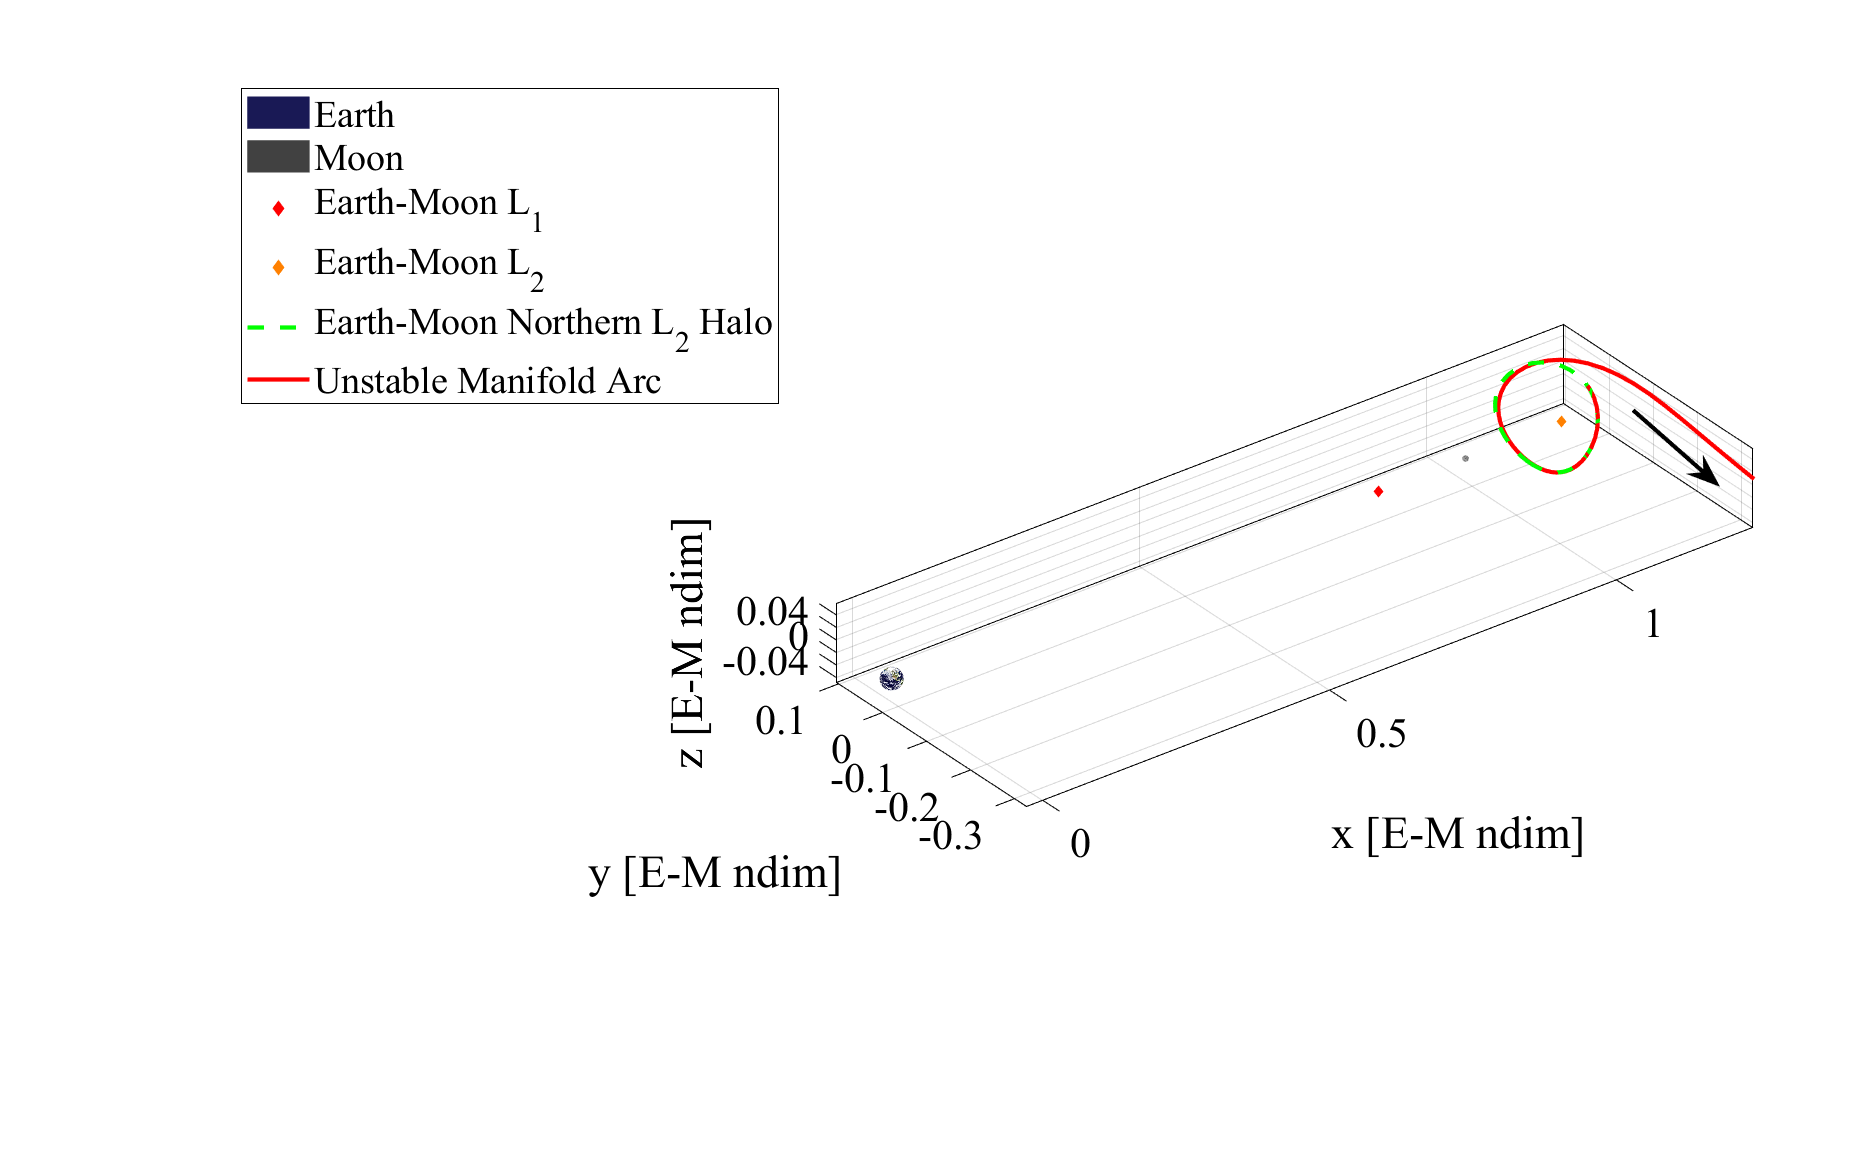
\includegraphics[width=0.9\textwidth]{figures/StagedMinTOFEM.pdf}
    \caption{Northern $L_{2}$ halo orbit ($JC=3.13$) departure manifold arc in the Earth-Moon barycentric rotating frame for a low-TOF case.}
    \label{fig:stagedMinTOFEM}
\end{figure}

\begin{figure}[!htb]
    \centering
    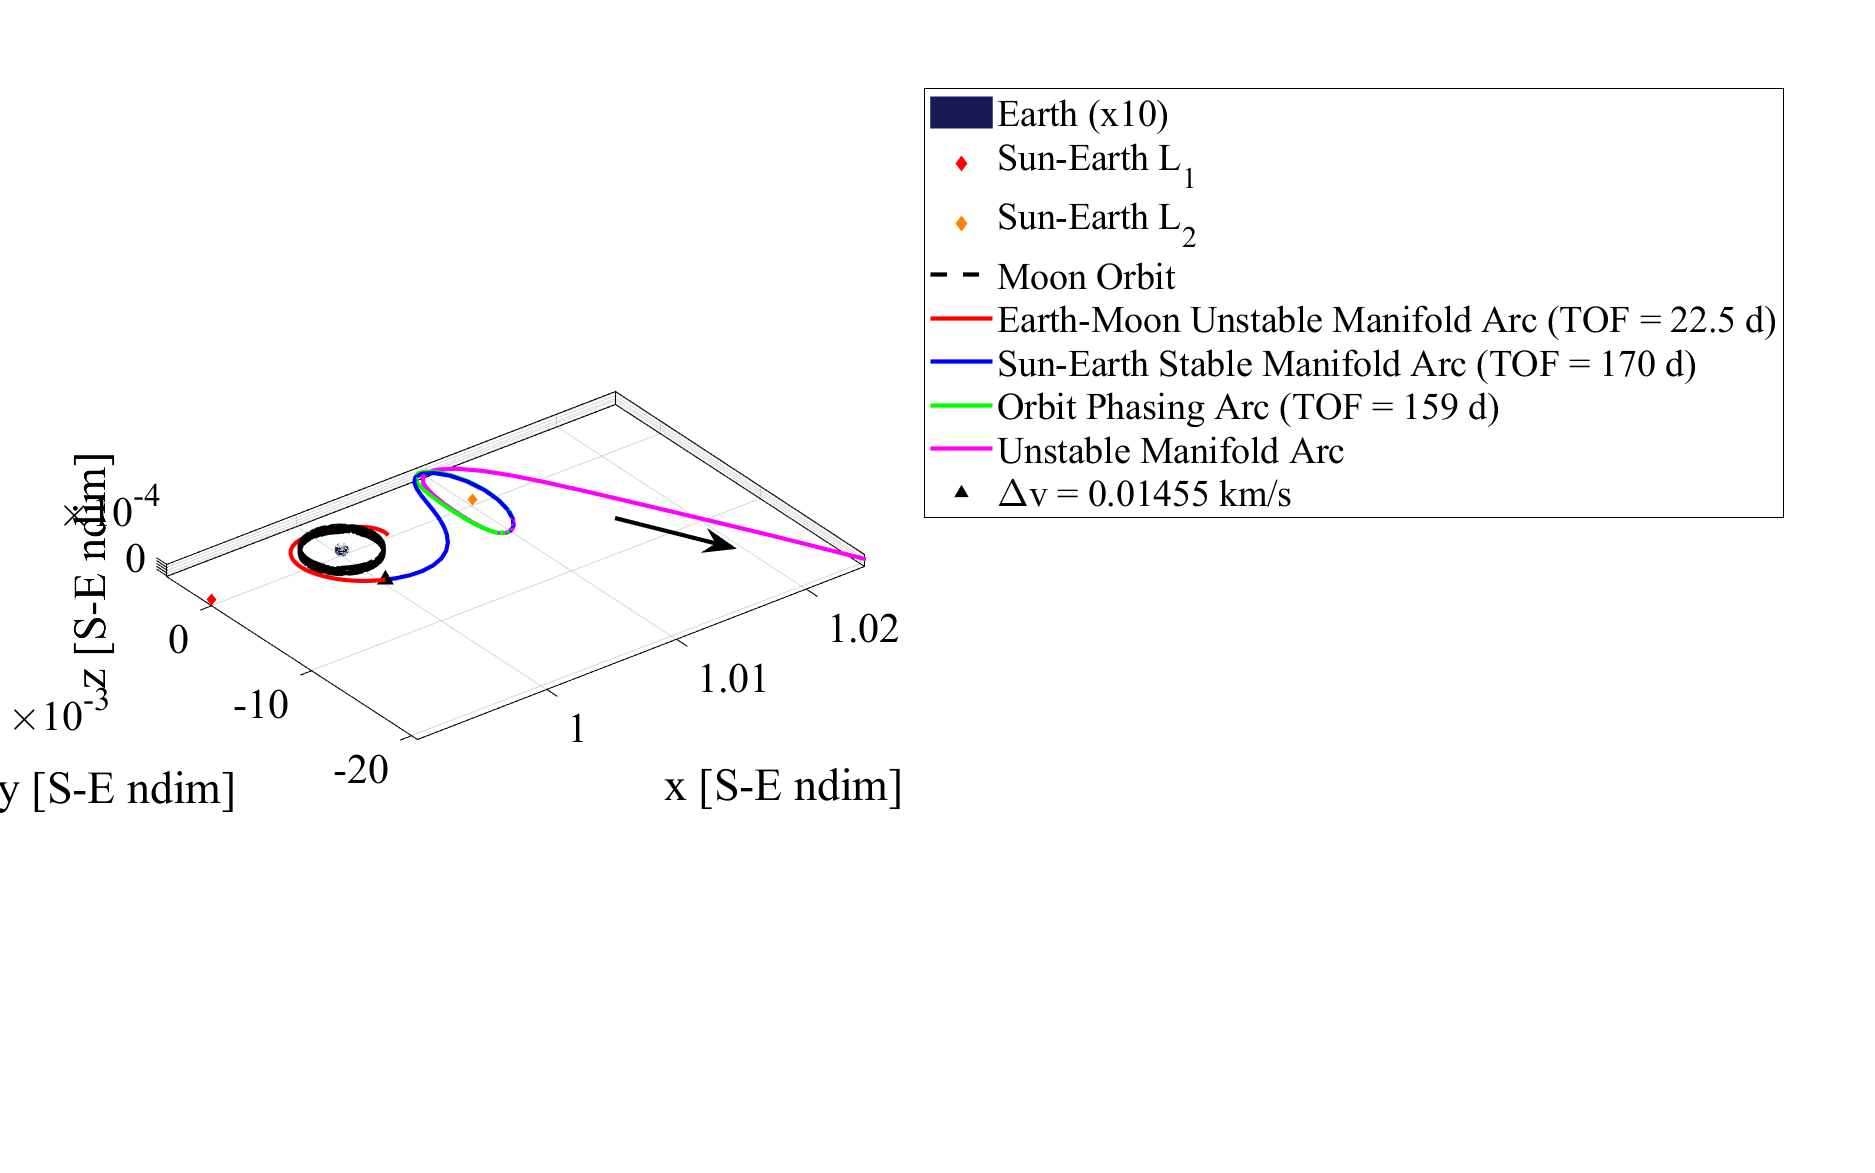
\includegraphics[width=0.9\textwidth]{figures/StagedMinTOFSE.pdf}
    \caption{Departure CR3BP arc with northern $L_{2}$ halo staging orbit ($JC=3.0008189$) in the Sun-Earth barycentric rotating frame for a low-TOF case.}
    \label{fig:stagedMinTOFSE}
\end{figure}

\begin{figure}[!htb]
    \centering
    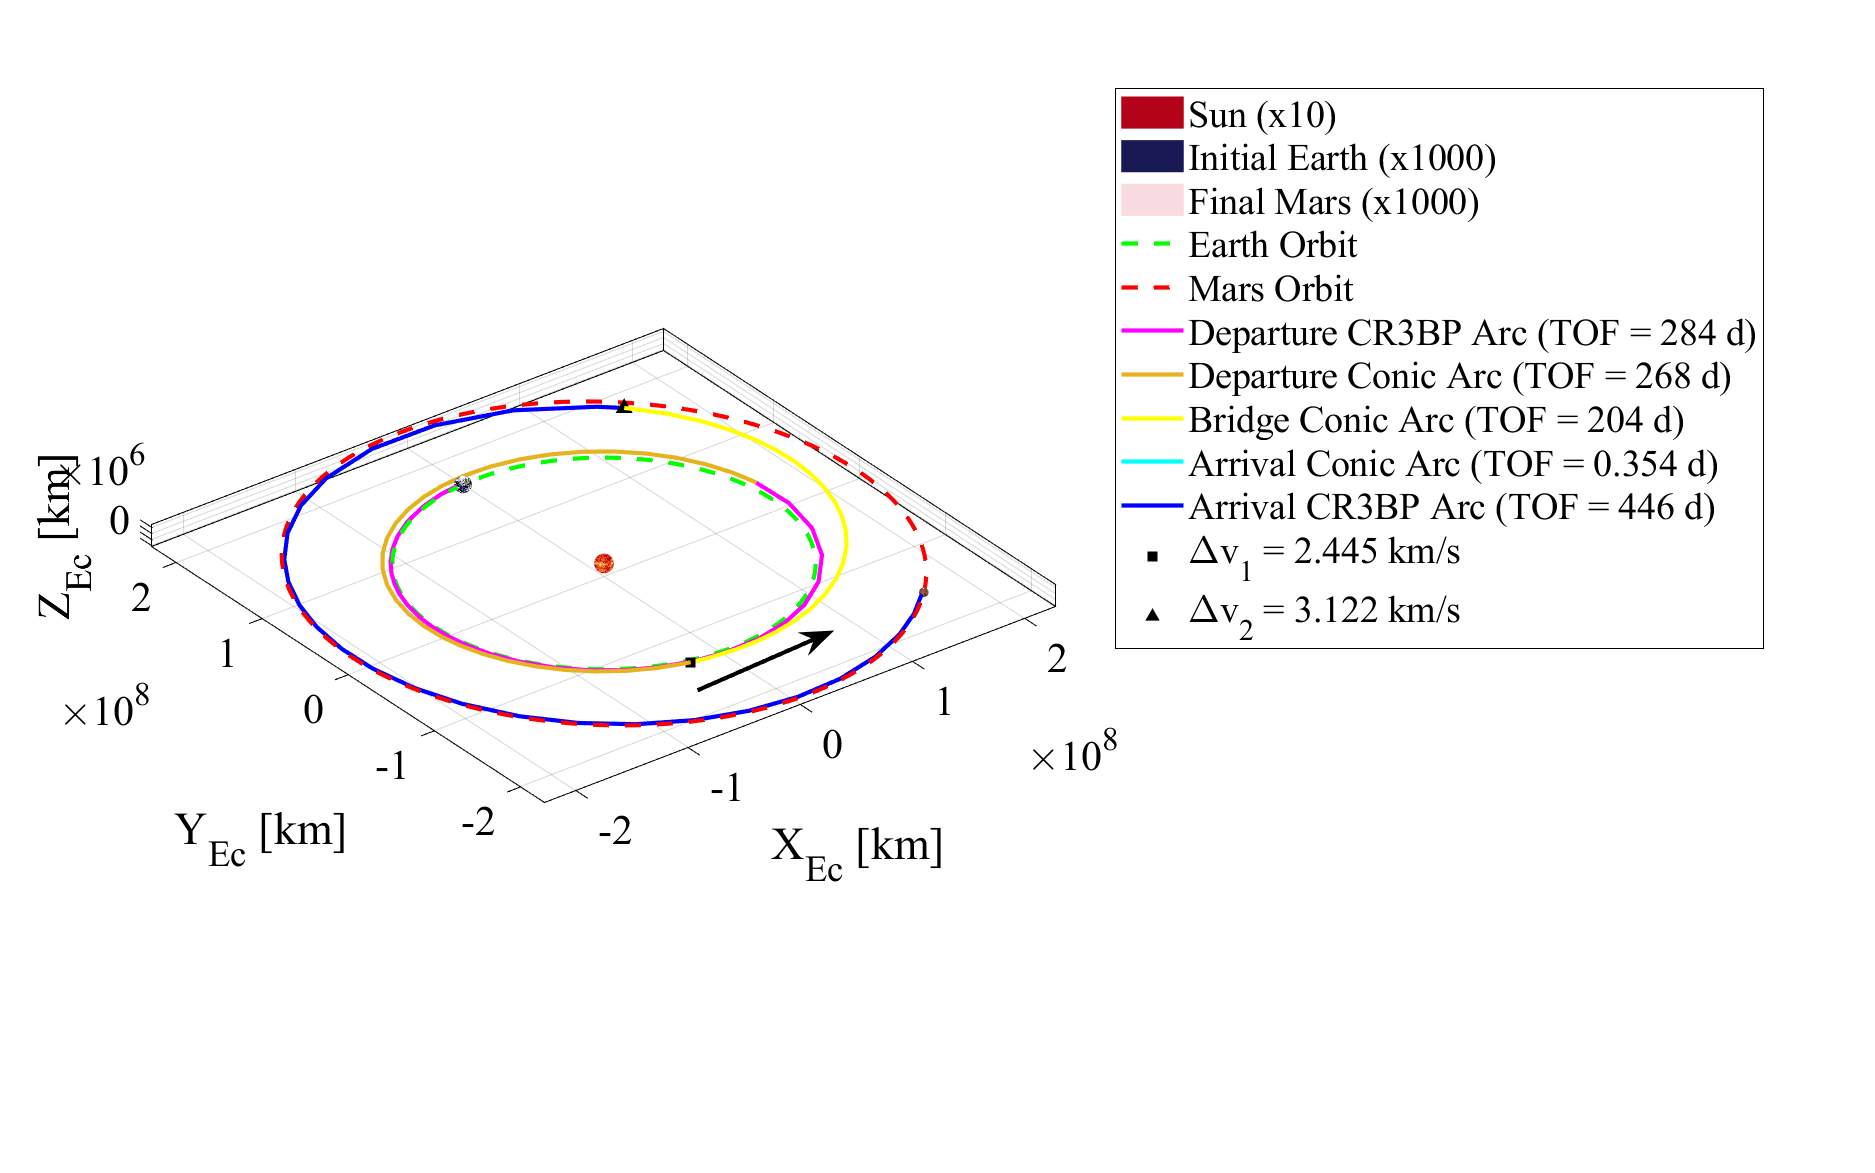
\includegraphics[width=0.9\textwidth]{figures/StagedMinTOFMMAT.pdf}
    \caption{MMAT in the Sun-centered Ecliptic J2000 frame for a staging orbit low-TOF case.}
    \label{fig:stagedMinTOFMMAT}
\end{figure}

\begin{figure}[!htb]
    \begin{subfigure}[h]{0.495\linewidth}
        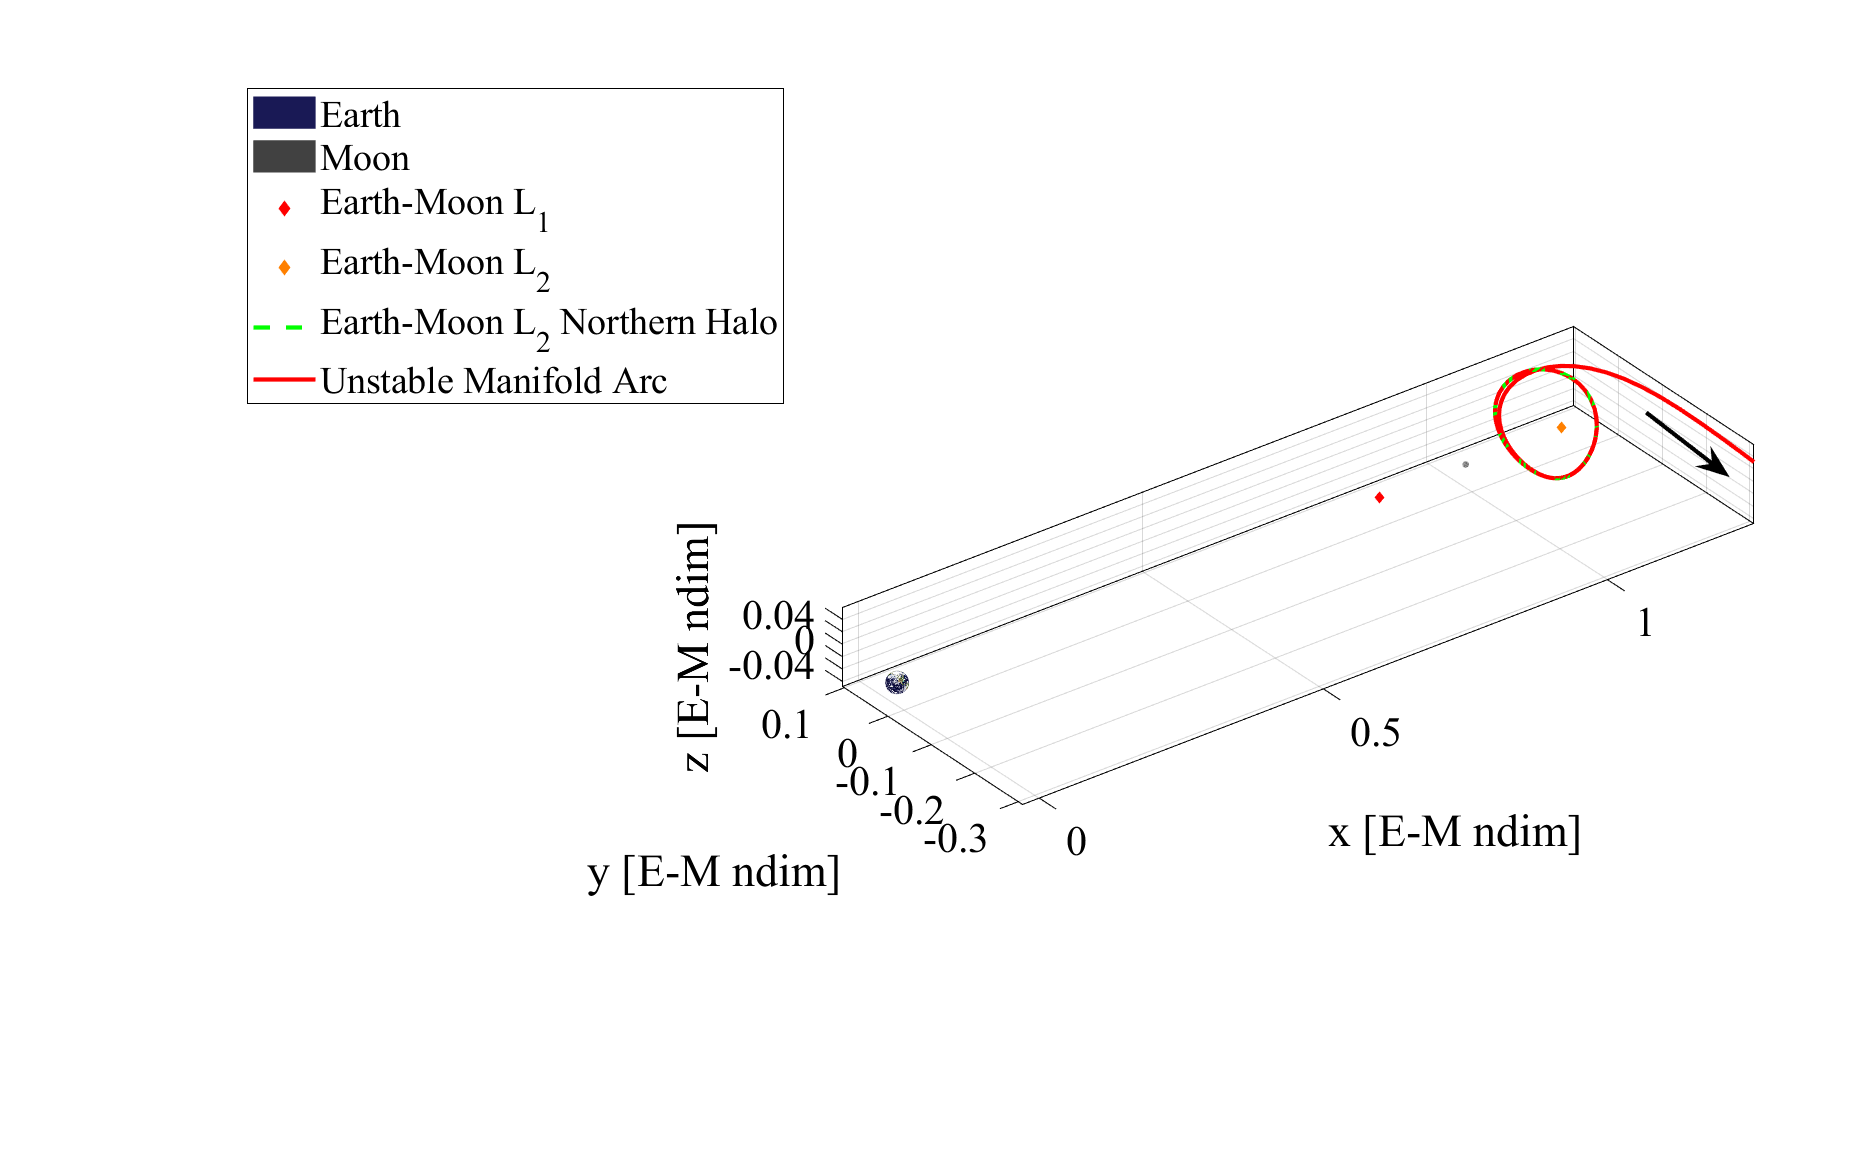
\includegraphics[width=\textwidth]{figures/DirectMinTOFEM.pdf}
        \caption{Earth-Moon barycentric rotating frame.}
    \end{subfigure}
    \hfill
    \begin{subfigure}[h]{0.495\linewidth}
        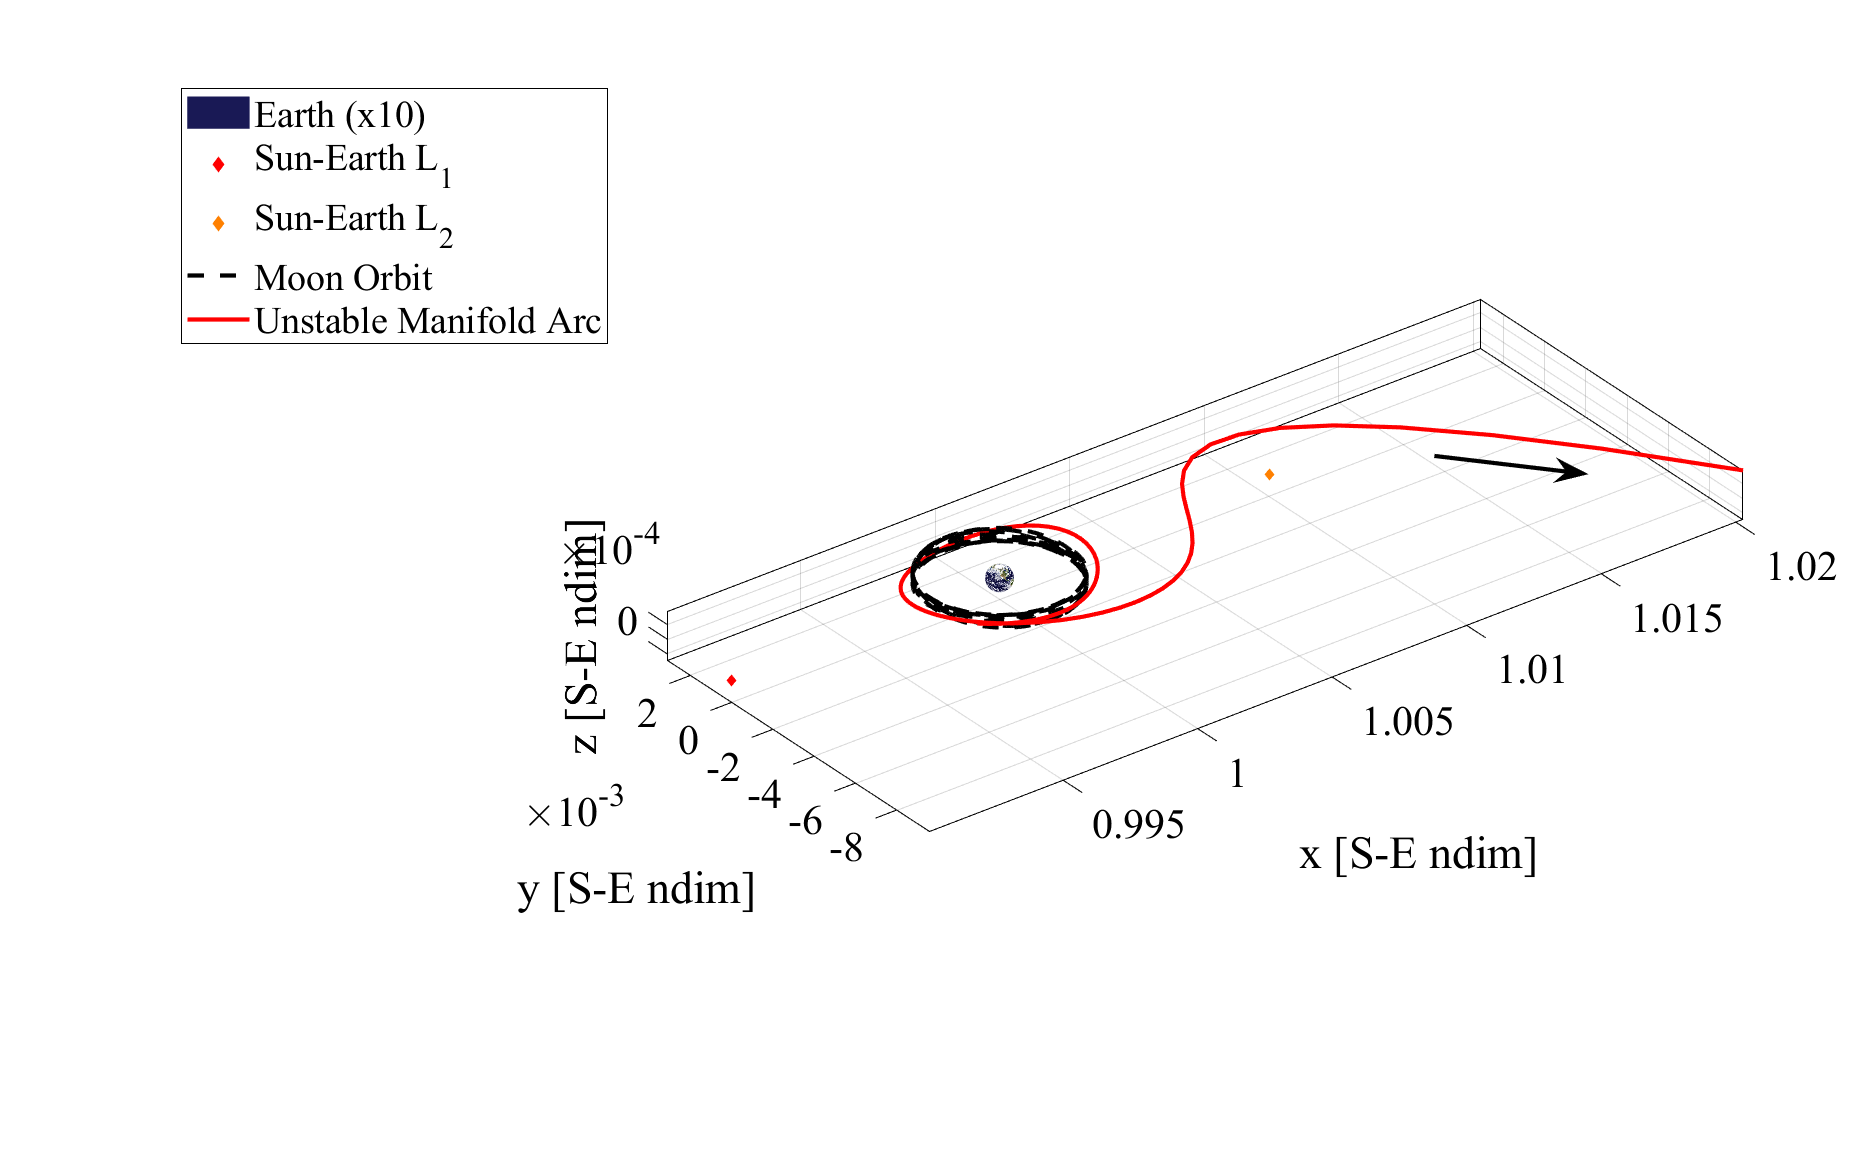
\includegraphics[width=\textwidth]{figures/DirectMinTOFSE.pdf}
        \caption{Sun-Earth barycentric rotating frame.}
    \end{subfigure}
    \caption{Northern $L_{2}$ halo orbit ($JC=3.13$) departure CR3BP arc for a low-TOF case.}
    \label{fig:directMinTOFE}
\end{figure}

\begin{figure}[!htb]
    \centering
    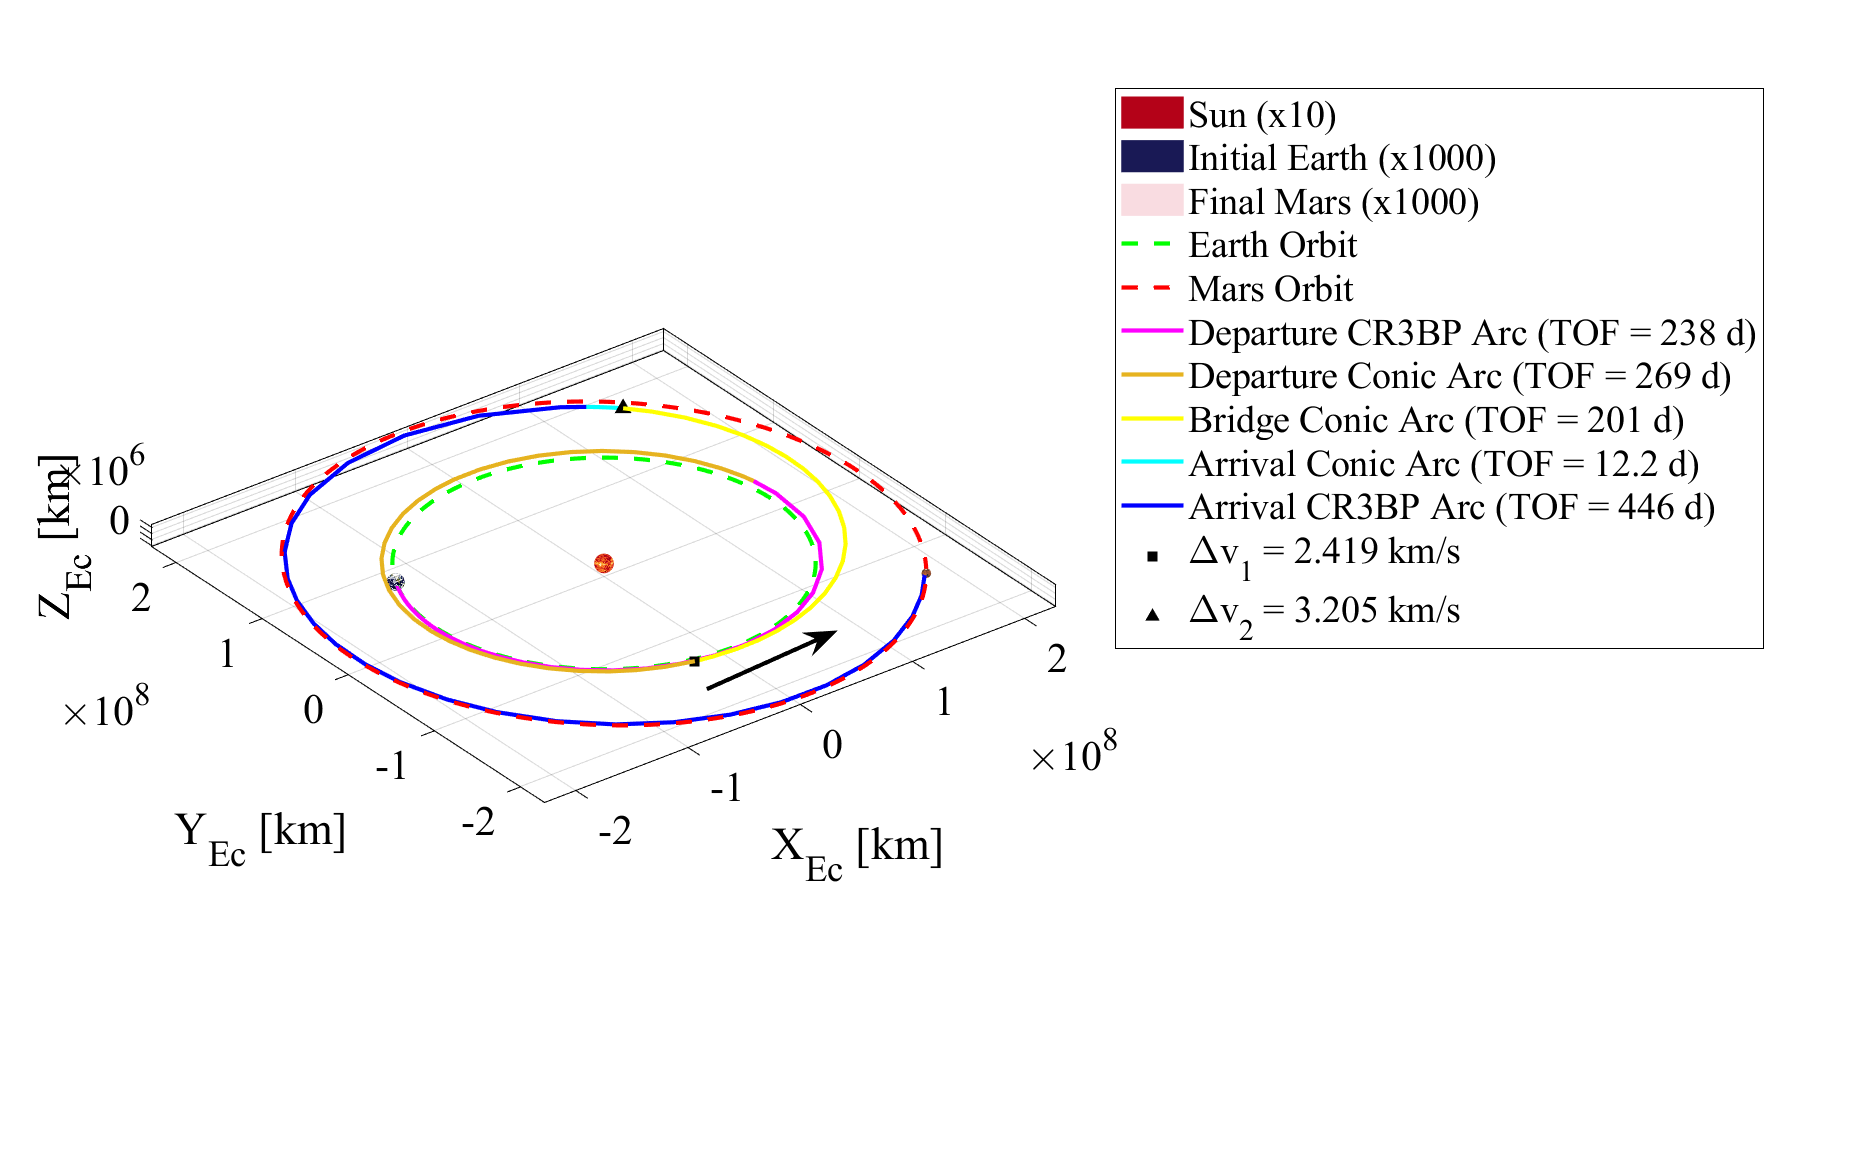
\includegraphics[width=0.9\textwidth]{figures/DirectMinTOFMMAT.pdf}
    \caption{MMAT in the Sun-centered Ecliptic J2000 frame for a direct low-TOF case.}
    \label{fig:directMinTOFMMAT}
\end{figure}

A few other ways to reduce the total transfer TOF involve the other three legs of the transfer.
Although the minimum-$\Delta v$ transfers occur when the bridge and arrival conic arc intersection
is $\ang{180}$ from the first MMAT maneuver, the bridge arc TOF can be decreased by moving the
final maneuver closer to the periapsis. While this will increase the maneuver cost, it can
sometimes be worth the flight time savings. Another option is to decrease the departure and arrival
CR3BP arc times-of-flight via the invariant manifold arc selections. Since some manifold arcs
depart faster from the system than others from the same orbit, this can lead to slight decreases in
TOF.

\subsection{Comparison between Departure Orbits}
Since both categories of transfers have similar average Maneuver $\Delta v$ costs among their
lowest-cost solutions, it is easiest to evaluate the two types separately for that metric.
\cref{fig:compareDeltavStaged} compares the average $\Delta v$ values for the lowest-cost
departures using staging orbits from the orbits used in this investigation. As mentioned
previously, no one orbit family performs the best across the range of Jacobi constant values;
however, some general trends can be identified. Overall, these transfers perform better than the
baseline modified Hohmann transfer in terms of maneuver cost by around $0.5$ km/s while at each
energy value, the spread between the families is on the order of $0.2$ km/s. Some families show
significant cost fluctuation across energy levels while others do not. The families that seem to
perform the best overall are the $L_{1}$ halo and $L_{1}$ vertical families, although they are not
necessarily the best choice at each Jacobi constant. The $L_{2}$ axial family also performs well,
but unfortunately, unstable members only exist at lower Jacobi constant values. While it may not be
the optimal choice in every mission scenario, the lowest maneuver cost staging orbit transfers in
this investigation originate from the $3.03$ $L_{1}$ northern halo orbit, with an average total
$\Delta v$ of $4.978$ km/s. \cref{fig:stagedMinDvEM}-\cref{fig:stagedMinDvMMAT} show one such
transfer from this specific departure orbit.

\begin{figure}[!htb]
    \centering
    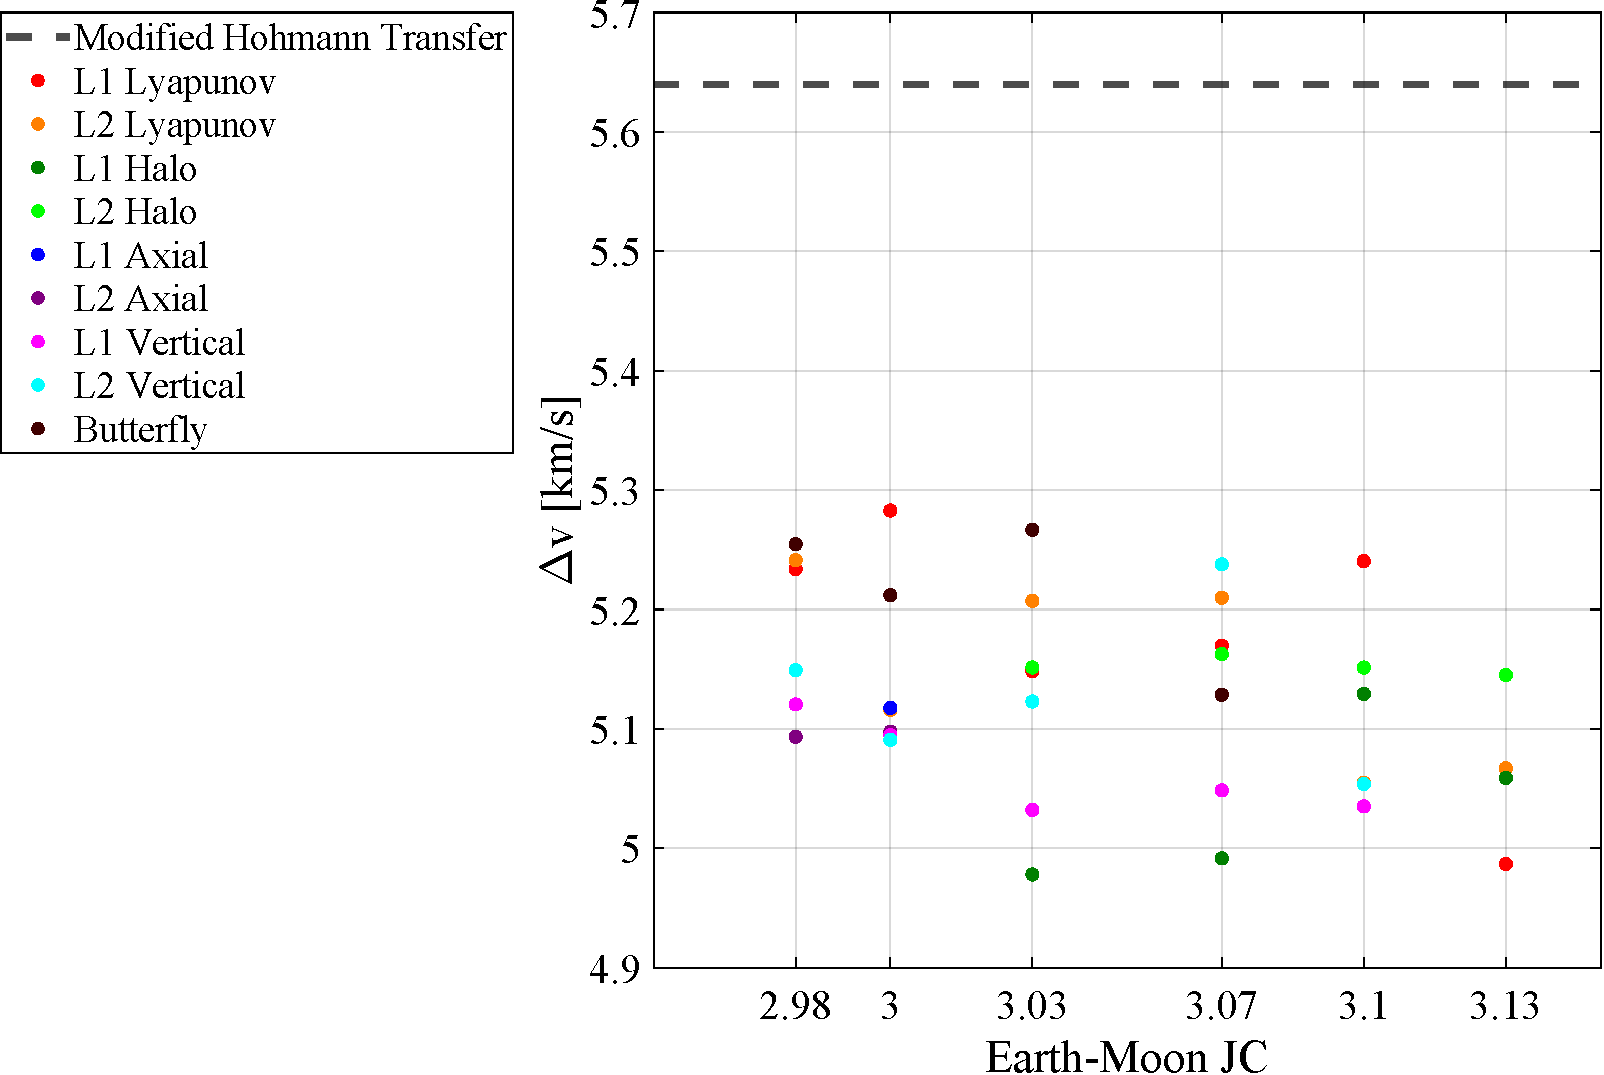
\includegraphics[width=0.9\textwidth]{figures/DeltavComparisonStaged.pdf}
    \caption{Average $\Delta v$ comparison between lowest-cost transfers with staging orbits from various orbits/families.}
    \label{fig:compareDeltavStaged}
\end{figure}

Similarly, \cref{fig:compareDeltavDirect} shows the average $\Delta v$ values for the lowest-cost
direct departures. These orbits display similar performance on average to the staging orbit
transfers in comparison to the baseline modified Hohmann transfer. However, the lowest $\Delta v$
cases reach nearly $0.8$ km/s improvement. The spread between the families is larger, reaching
$0.5$ km/s for some Jacobi values, but the variation across families is just as inconsistent as
with the staging orbit transfers. For these direct transfers, the $L_{1}$ Lyapunov orbit family
performs the best by far at every Jacobi constant value except $3.1$ (where it is one of the worst
options). The $L_{1}$ halo family also performs well overall. The $3.0$ $L_{1}$ Lyapunov orbit
provides the lowest maneuver cost direct transfer with an average total $\Delta v$ of $4.791$ km/s.
An example transfer from this orbit is shown in \cref{fig:directMinDvE} and
\cref{fig:directMinDvMMAT}.

\begin{figure}[!htb]
    \centering
    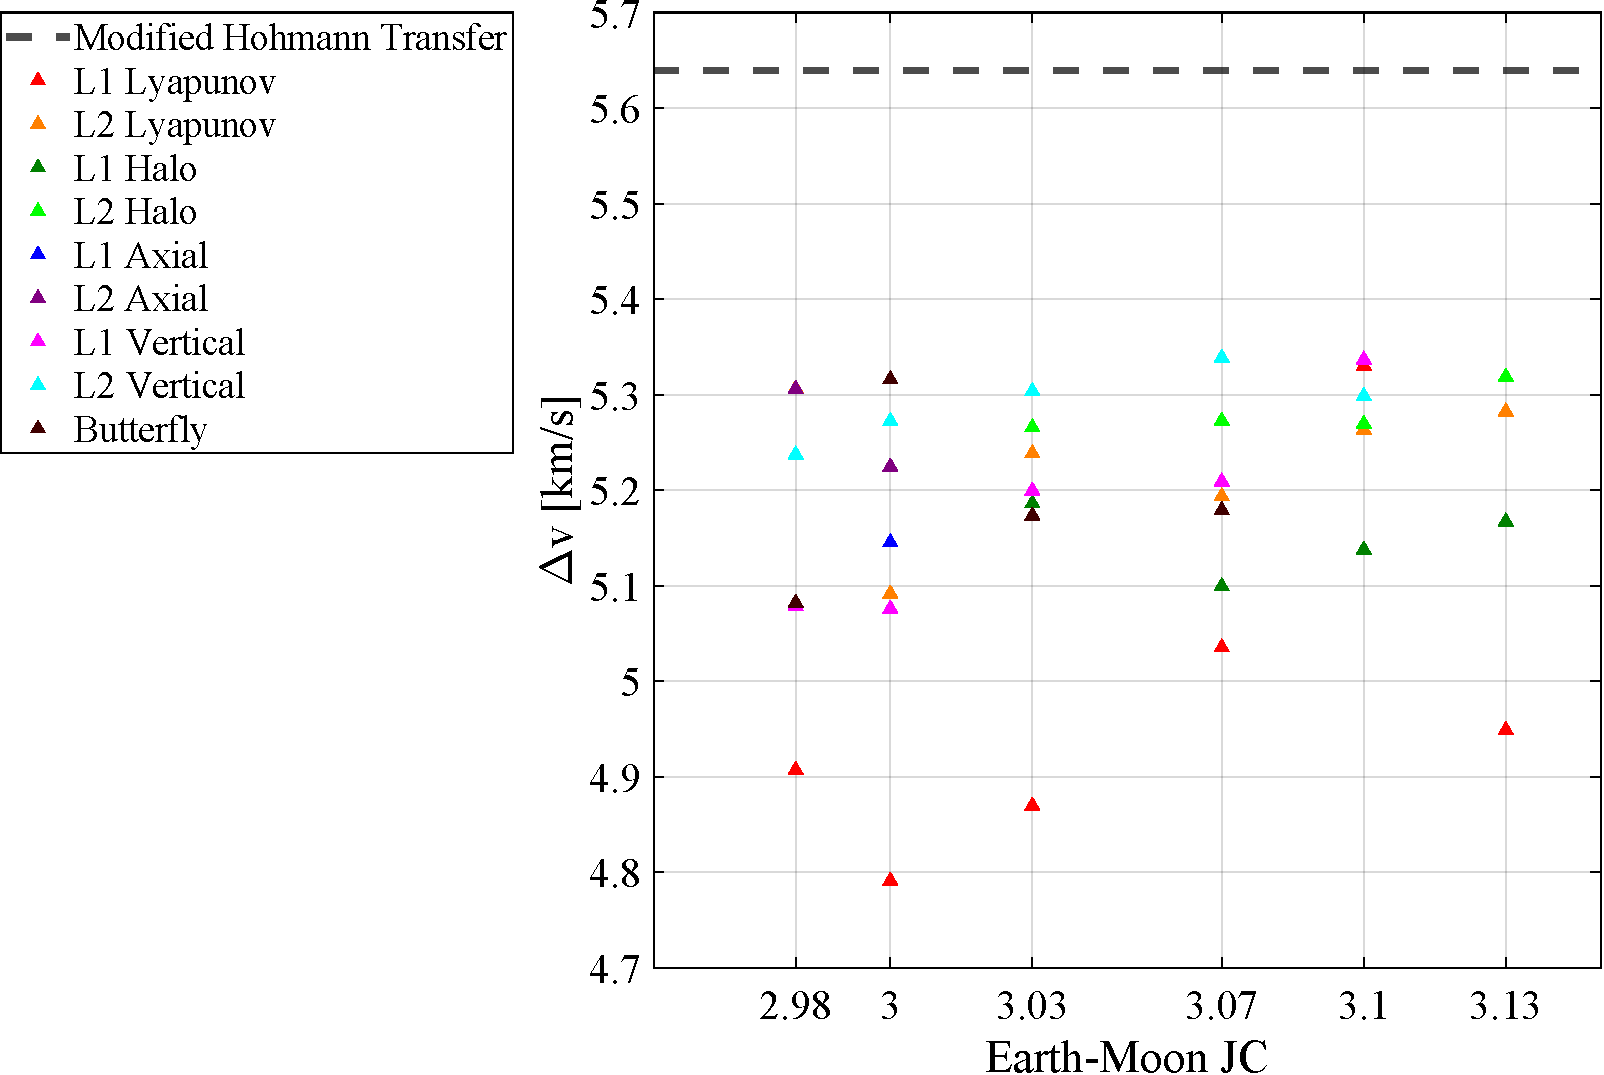
\includegraphics[width=0.9\textwidth]{figures/DeltavComparisonDirect.pdf}
    \caption{Average $\Delta v$ comparison between lowest-cost transfers with direct departures from various orbits/families.}
    \label{fig:compareDeltavDirect}
\end{figure}

For both categories of transfers, $L_{1}$ orbit families seem to produce lower-$\Delta v$
transfers. It is likely that many of these transfers with invariant manifolds originating from
Earth-Moon $L_{1}$ departure families leverage close passes by the Moon to lessen the eventual
energy gap between the planetary systems, resulting in decreased maneuver costs. Again comparing
the two transfer types, in general, the lowest-cost transfers with direct departures outperform the
lowest-cost transfers with staging orbits in terms of maneuver costs. Nevertheless, both types see
cost reduction compared to the baseline modified Hohmann transfer.

When comparing the total transfer TOF between the two categories, the differences are large enough
to be evaluated directly in a single figure. \cref{fig:compareTOF} shows the average lowest-cost
TOF values for both staging orbit transfers and those with direct departures. The staging orbit
transfers all lie in the range of $4.7$-$5.5$ years, while the direct transfer times-of-flight are
significantly lower in comparison: $3.9$-$4.6$ years. It is interesting to note that the energy
levels with higher times-of-flight for the staging orbit transfers are not the same as the higher
TOF options for direct transfers. The spread in TOF between the families at each Jacobi constant
value fluctuates both within each transfer type and overall. For instance, the $3.1$ direct
transfers have a spread of about $0.15$ years while it is $0.6$ at a Jacobi constant of $2.98$, and
the spread is near $0.3$ years for staged orbits at a Jacobi constant of $3.03$ but $0.6$ years for
$3.07$.

\begin{figure}[!htb]
    \centering
    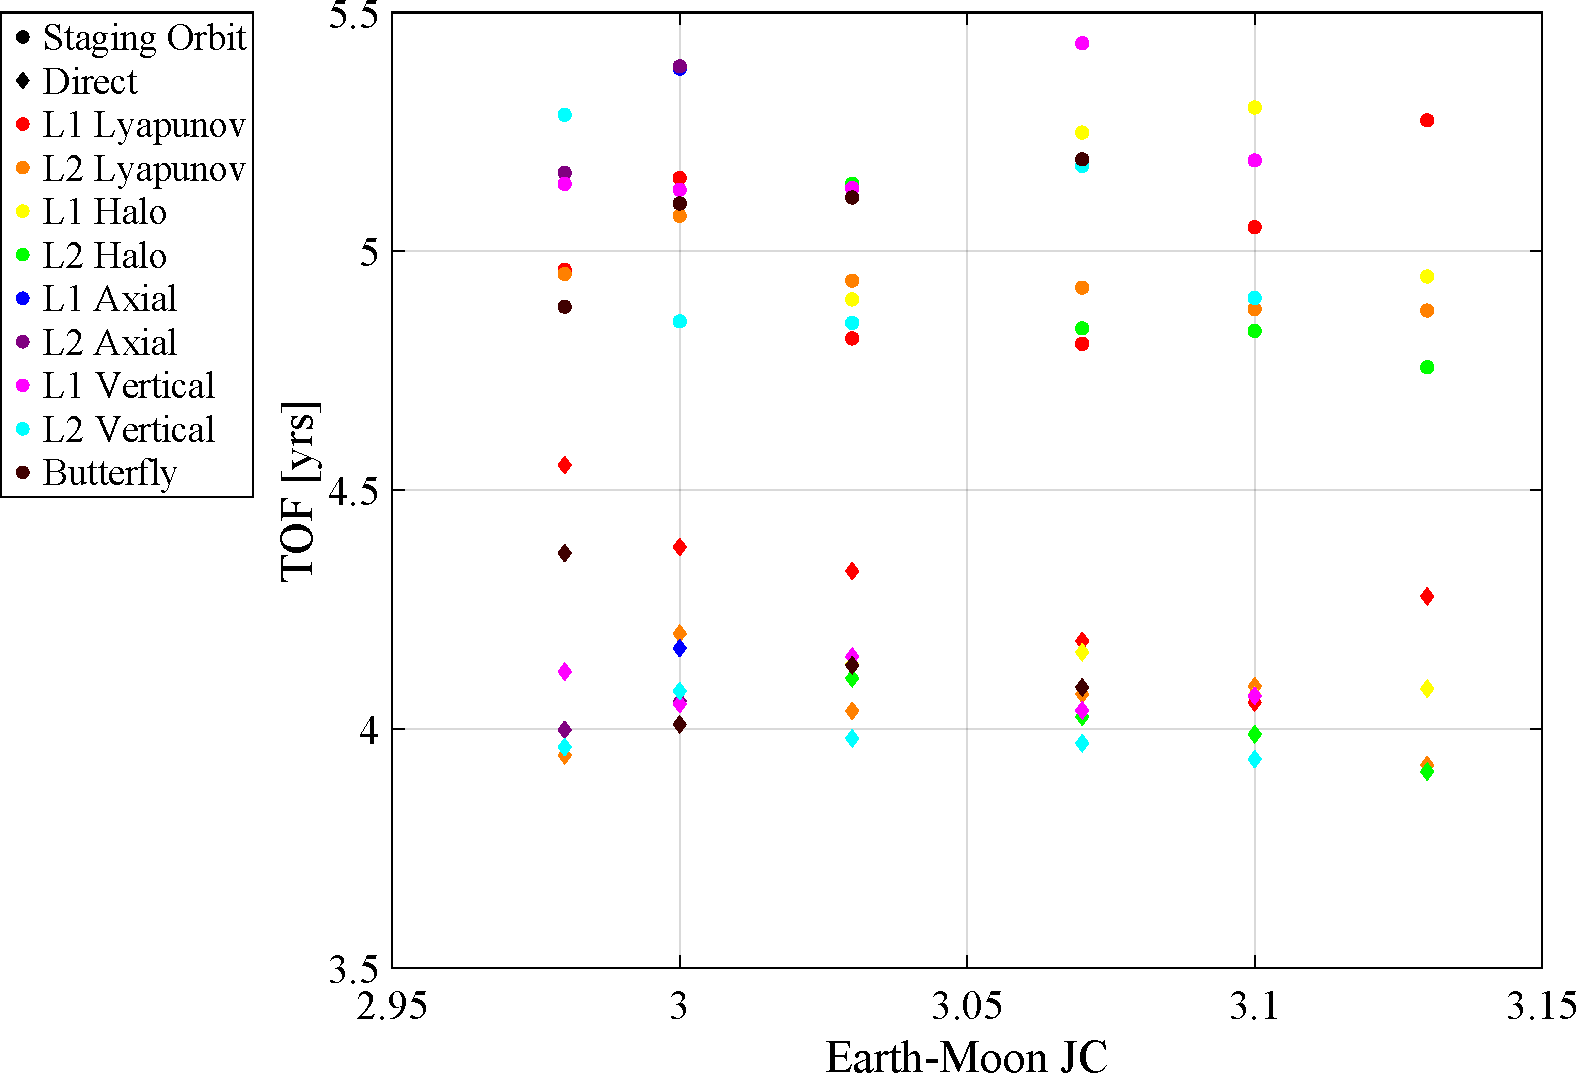
\includegraphics[width=0.9\textwidth]{figures/TOFComparison.pdf}
    \caption{Average TOF comparison between lowest-cost transfers from various orbits/families.}
    \label{fig:compareTOF}
\end{figure}

Like with the total $\Delta v$ costs, the lowest-cost total TOF values fluctuate unpredictably
across each family of orbits. Regardless, for the transfers with staging orbits, the $L_{2}$
Lyapunov and $L_{2}$ halo orbits perform the best overall in TOF, although the results are a little
less clear than when comparing $\Delta v$ costs. The lowest TOF option investigated is the $3.13$
$L_{2}$ northern halo orbit, with an average total TOF of $4.76$ years, shown in
\cref{fig:stagedMinTOFEM}-\cref{fig:stagedMinTOFMMAT}. For the direct transfers, the $L_{2}$ halo
and $L_{2}$ butterfly orbits have the lowest times-of-flight. The $L_{2}$ axial orbits also perform
well at their limited energy values as before. In this category, the $3.13$ $L_{2}$ northern halo
orbit again performs the best with an average total TOF of $3.91$ years, shown in
\cref{fig:directMinDvE} and \cref{fig:directMinDvMMAT}. While $L_{1}$ departure orbits seem to
provide lower maneuver costs, \cref{fig:compareTOF} shows that $L_{2}$ departure orbits tend to
have lower lowest-cost times-of-flight. This may be because the manifold arcs reach the Earth SoI
faster and extend slightly farther, decreasing the TOF of the transfer.

Many of the previous examples have shown that the transfers with lower total $\Delta v$ tend to
have higher times-of-flight and vice versa. Therefore, to find the departure orbits that provide
decreases in both, the lowest-cost solutions are compared using $J$, the cost function value. The
results of this comparison are shown in \cref{fig:compareJ}. Immediately, it is clear once again
that the transfers with direct departures outperform those with staging orbits, with $J$ values
near $31$ and $36$ respectively. Note that these $J$ values have little physical significance but
are a linear combination of the $\Delta v$ and TOF. The $J$ value spread at each Jacobi constant
value is similar to the spread in TOF in \cref{fig:compareTOF}.

\begin{figure}[!htb]
    \centering
    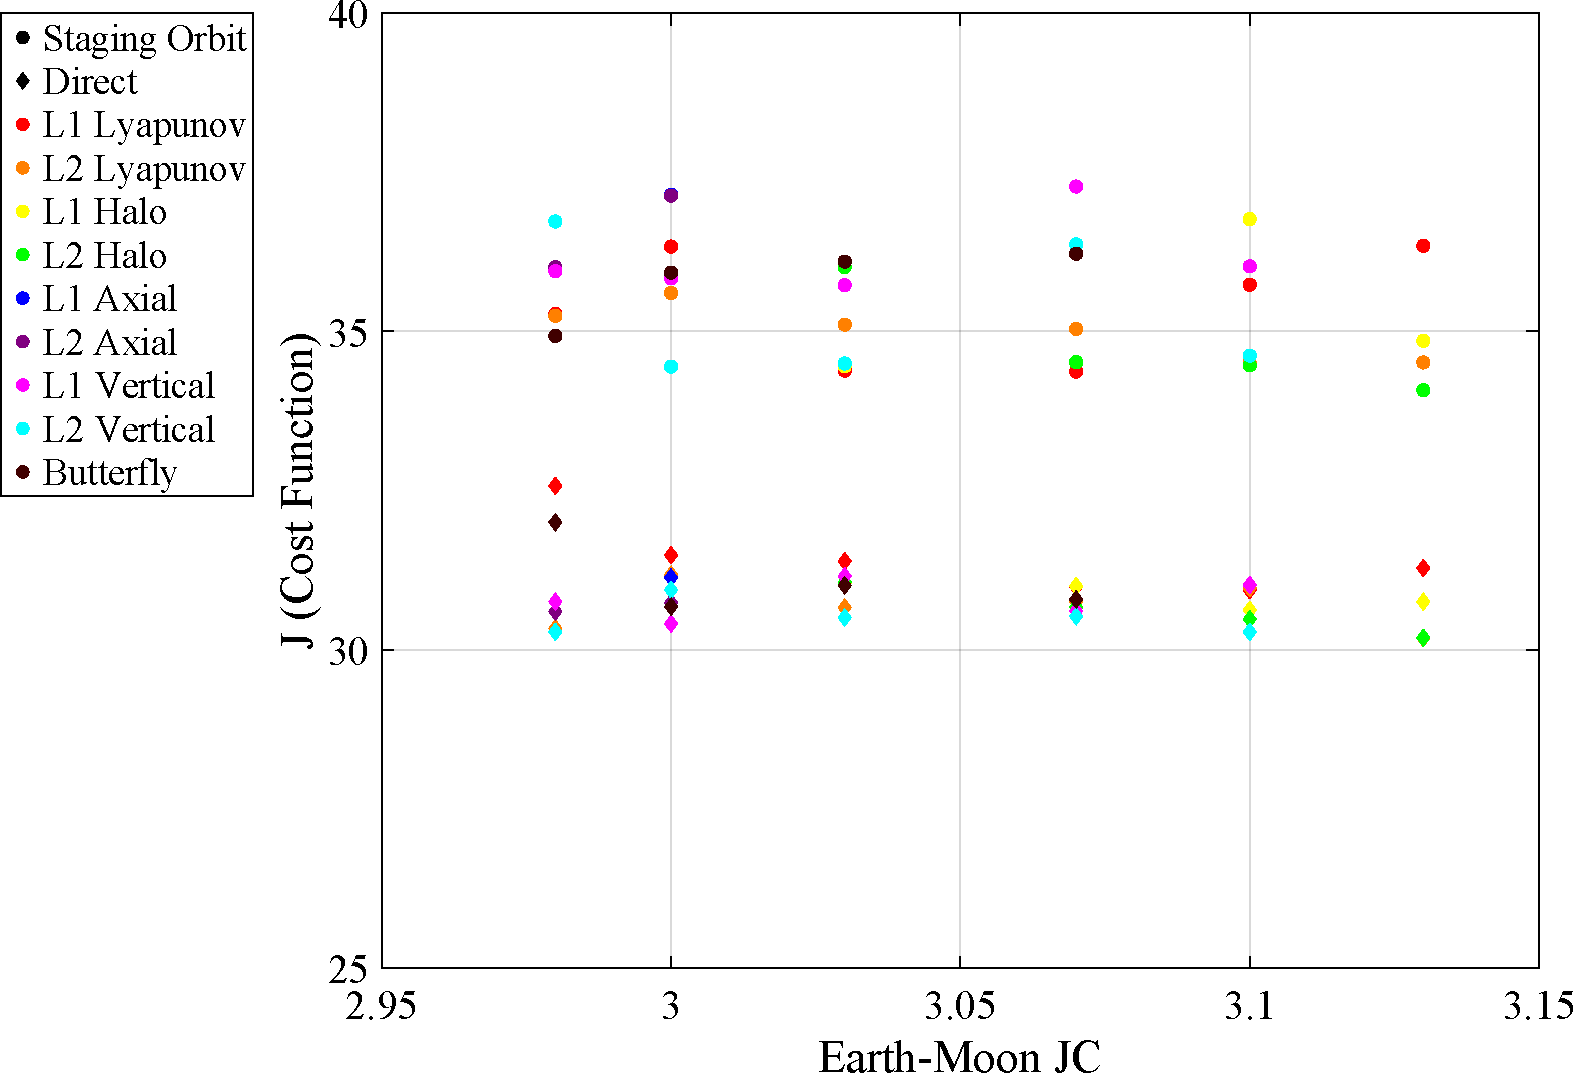
\includegraphics[width=0.9\textwidth]{figures/JComparison.pdf}
    \caption{Average cost function value comparison between lowest-cost transfers from various orbits/families.}
    \label{fig:compareJ}
\end{figure}

In general, comparing the $J$ values between the departure orbits, it is less clear which families
perform the best. For the staging orbits, the $L_{2}$ halo orbits have lower costs at the higher
Jacobi constant values. At the lower Jacobi constants, the better families are different for each
case, although the $L_{2}$ Lyapunov orbits are consistently low throughout. Comparing the direct
transfers, the $L_{2}$ vertical orbit family performs well across the majority of the energy range,
with the $L_{2}$ halos again having low values at higher Jacobi constant orbits. The lowest overall
cost departure orbit is surprisingly the $3.13$ $L_{2}$ Lyapunov orbit direct departure, with an
average cost function value of $30.19$, an average total maneuver cost of $5.282$ km/s, and an
average total TOF of $3.92$ years. The lowest-cost direct transfer from this departure orbit is
shown in \cref{fig:bestE} and \cref{fig:bestMMAT} with a total maneuver cost of $5.293$ km/s and
TOF of $3.24$ years.

\begin{figure}[!htb]
    \begin{subfigure}[h]{0.495\linewidth}
        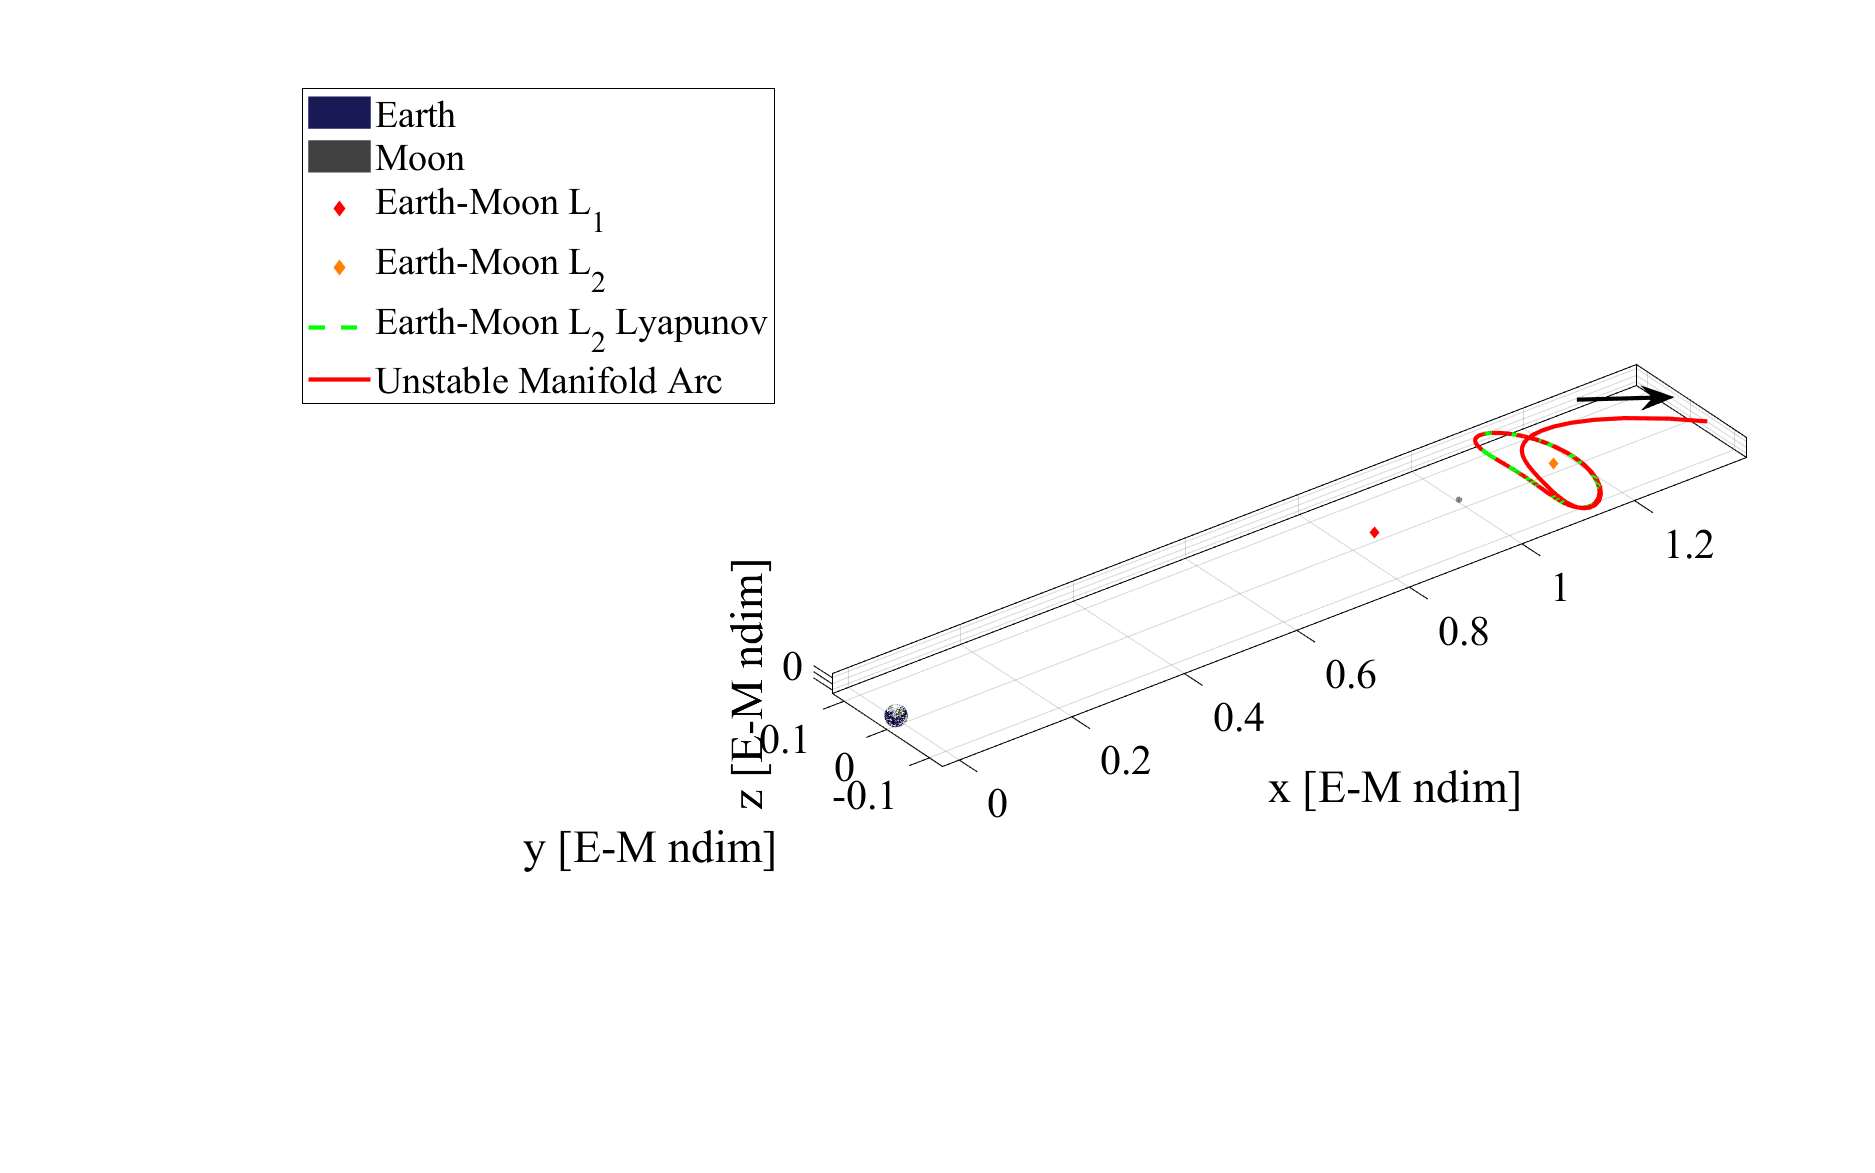
\includegraphics[width=\textwidth]{figures/BestEM.pdf}
        \caption{Earth-Moon barycentric rotating frame.}
    \end{subfigure}
    \hfill
    \begin{subfigure}[h]{0.495\linewidth}
        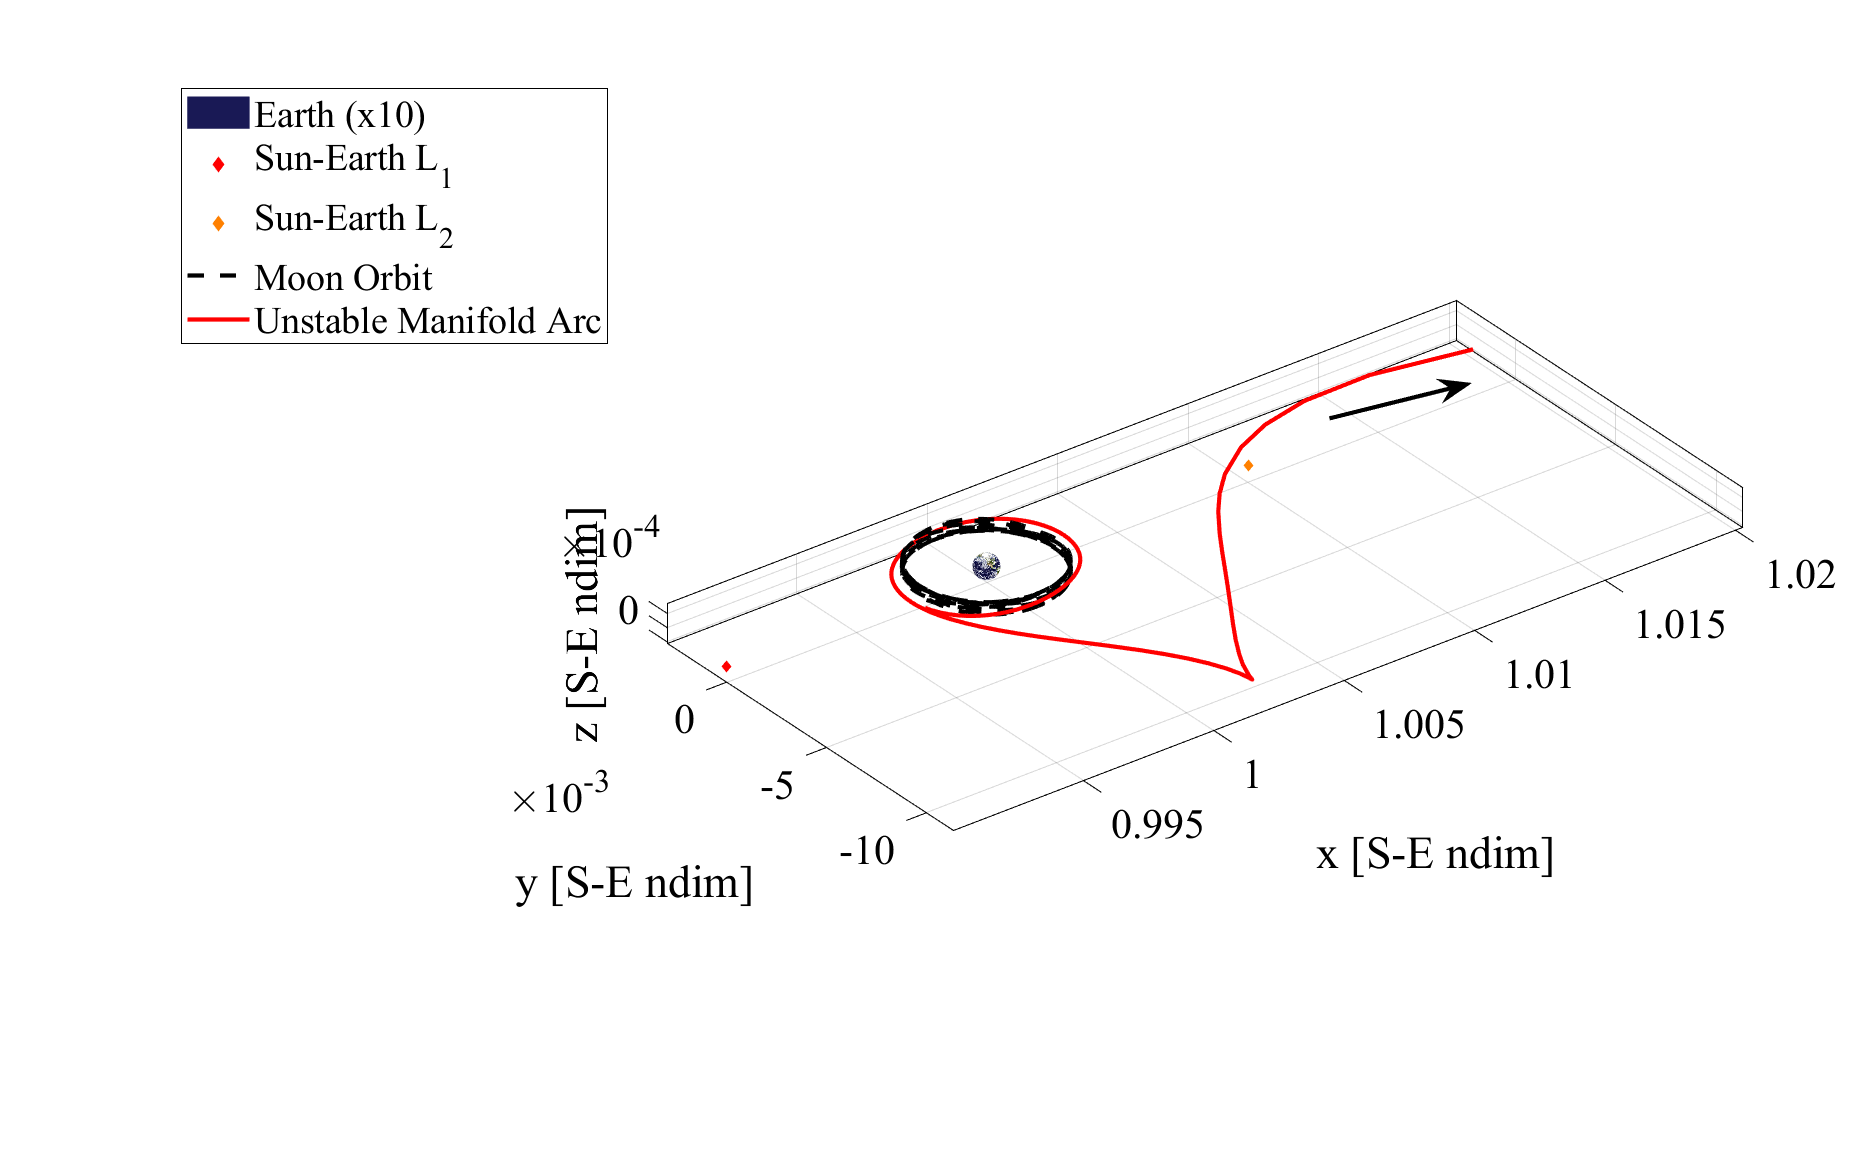
\includegraphics[width=\textwidth]{figures/BestSE.pdf}
        \caption{Sun-Earth barycentric rotating frame.}
    \end{subfigure}
    \caption{$L_{2}$ Lyapunov orbit ($JC=3.13$) departure CR3BP arc for lowest-cost case.}
    \label{fig:bestE}
\end{figure}

\begin{figure}[!htb]
    \centering
    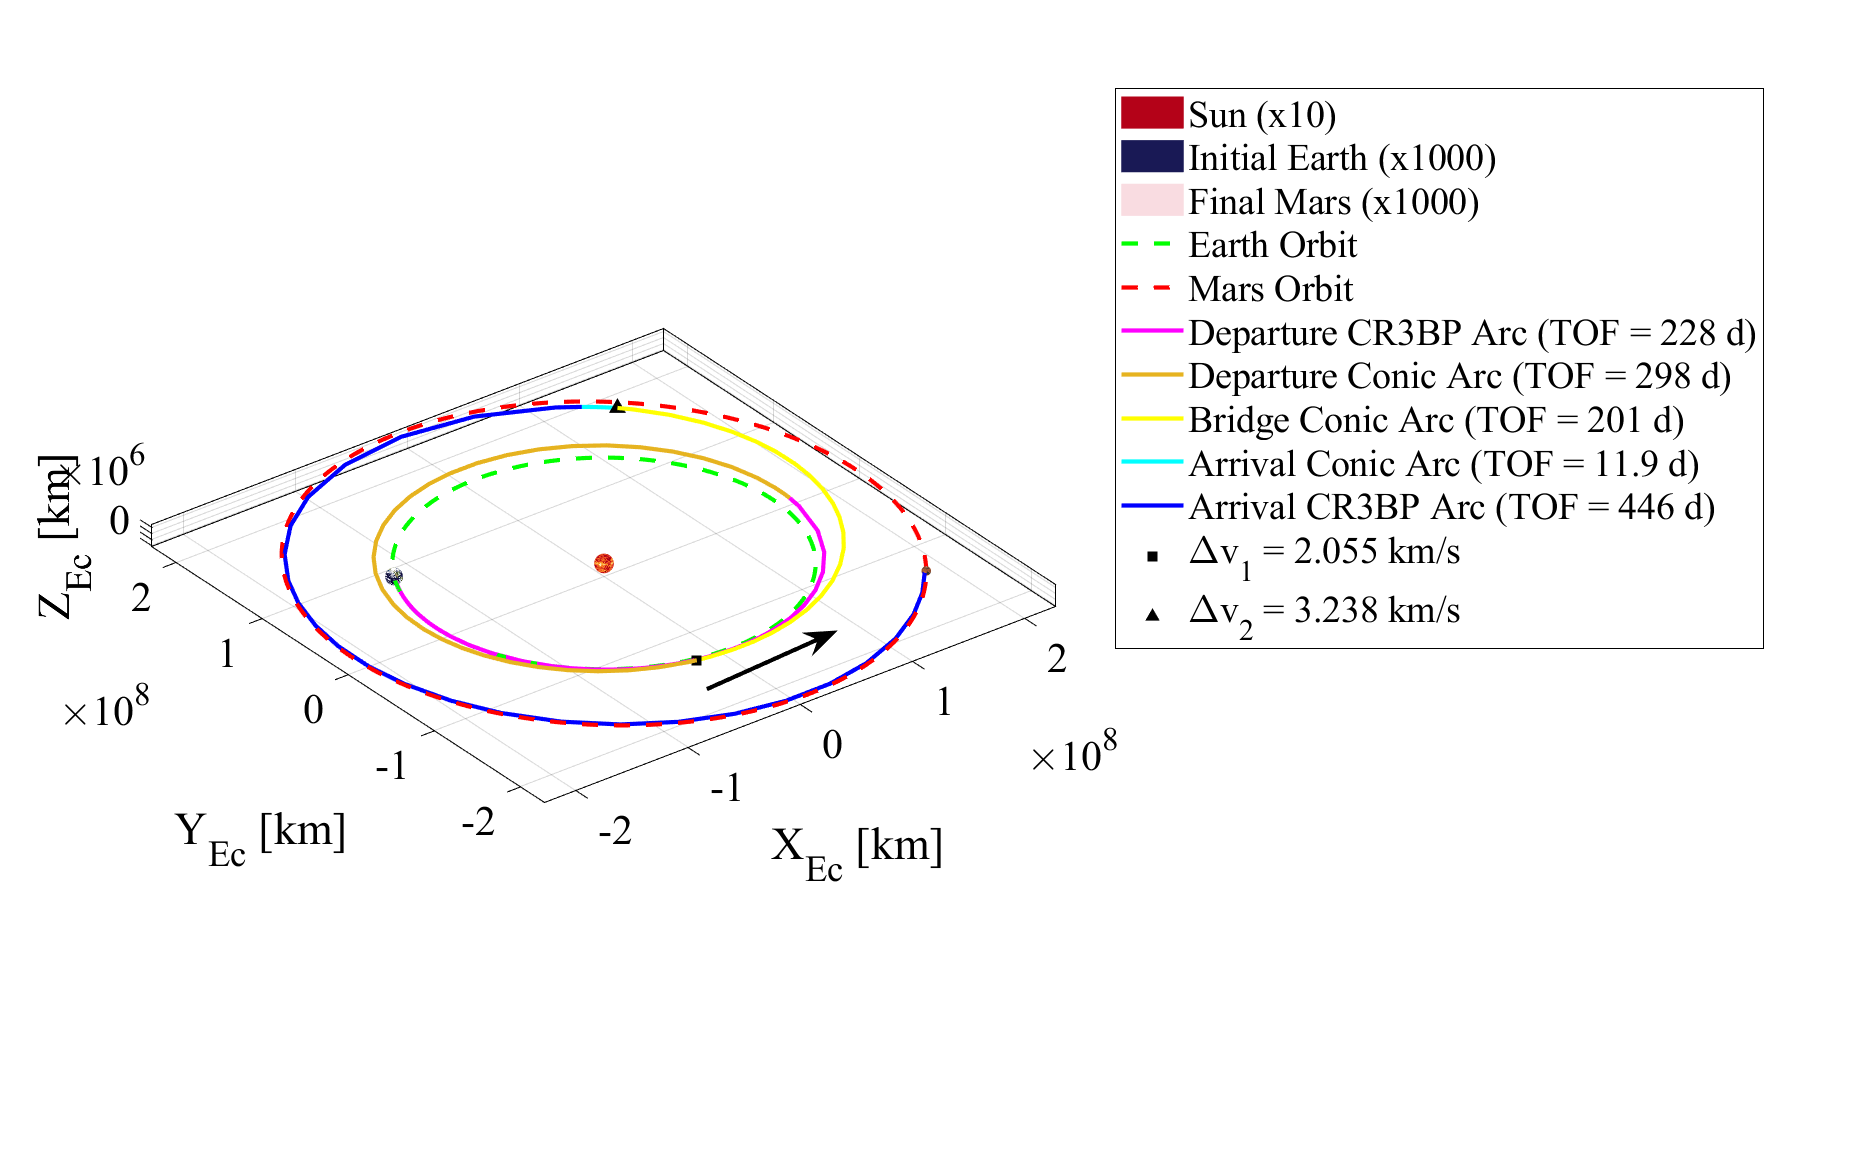
\includegraphics[width=0.9\textwidth]{figures/BestMMAT.pdf}
    \caption{MMAT in the Sun-centered Ecliptic J2000 frame for lowest-cost case.}
    \label{fig:bestMMAT}
\end{figure}

\section{Comparison to Previous Work}\label{sec:PreviousWork}
As mentioned previously, several authors have investigated transfers between Earth or cislunar
space and Mars. The studies employ a variety of methodologies to accomplish their transfers,
leveraging direct impulsive burns, low-thrust, and/or invariant manifolds. Some of their relevant
findings are provided here for comparison to the results of this investigation. It is important to
note that each of the transfers from these investigations, whose results are consolidated into
\cref{tab:transferCosts}, utilizes a different methodology. Some employ an optimizer, others
leverage invariant manifolds, and the number and placement of maneuvers vary from transfer to
transfer. Additionally, each one departs from and arrives at different locations, making it
difficult to directly compare the total maneuver cost and TOF values. Many of the investigations
also assume that the orbital planes of Earth and Mars are coplanar, neglecting the nontrivial plane
change maneuver required when considering true orbital planes. Consequently, a direct comparison
cannot be made between all of the methodologies. However, they do provide some intuition for the
costs of similar interplanetary transfer types.

Kakoi et al. inspires the transfer methodology between the Earth-Moon and Sun-Earth CR3BP
models in this investigation\cite{Kakoi:2014,Kakoi:2015}. Their investigation focused on comparing
different transfer scenarios departing from Earth-Moon $L_{1}$ and $L_{2}$ halo orbits. While the
strategies employed are slightly different, Kakoi et al. construct transfers that utilize Sun-Earth
unstable invariant manifold arcs and compare them to direct transfers from Earth-Moon halo orbits.
As some sample values for an $L_{2}$ halo departure, their investigation found that a transfer
along a Sun-Earth halo unstable manifold arc required a total maneuver cost of $1.604$ km/s and a
total TOF of $1762$ days ($4.82$ years). Note that in their investigation, a maneuver is applied
along the departure manifold arc to speed up the transfer and the final destination is the
ephemeris location of Mars, cutting off the long arrival time of the stable manifold arc. On the
other hand, directly utilizing an unstable manifold arc from the Earth-Moon halo orbit resulted in
a transfer with a $\Delta v$ of $0.921$ km/s and a TOF of $1784$ days ($4.88$
years)\cite{Kakoi:2015}. The direct transfer again employs a maneuver along the departure manifold
arc, as well as an inclination change maneuver during an Earth-flyby. Other direct transfers
provided in the study have lower and higher times-of-flight and maneuver costs, demonstrating that
there are a wide variety of available transfer options.

\begin{table}[H]
    \centering
    \caption{Representative transfer costs from previous and current investigations.}
    \begin{tabular}{|c|c|c|c|c|}
        \hline
        \textbf{Transfer Type}                      &   \textbf{Origin} &   \textbf{Destination}    &   \boldmath$\Delta v$ \textbf{[km/s]} &   \boldmath$TOF$ \textbf{[days]}  \\  \hline
        Hohmann Transfer                            &   Earth           &   Sun-Mars $L_{1}$        &   5.64                                &   258                             \\  \hline
        Lambert Arc\cite{Eagle:2022}                &   Earth           &   Mars                    &   5.61                                &   310                             \\  \hline
        Optimized 4-Body\cite{Miele:1999}           &   LEO             &   LMO                     &   5.65                                &   258                             \\  \hline
        Lambert Arc CR3BP\cite{Conte:2017}          &   Lunar DRO       &   LMO                     &   3.29                                &   206                             \\  \hline
        CR3BP Manifolds\cite{Topputo:2005}          &   S-E Lyapunov    &   S-M Lyapunov            &   3.76                                &   999                             \\  \hline
        Pseudo-Manifolds\cite{Haibin:2014}          &   S-E Halo        &   S-M Halo                &   2.06                                &   596                             \\  \hline
        CR3BP Manifolds\cite{Kakoi:2014}            &   E-M Halo        &   Mars                    &   0.92                                &   1784                            \\  \hline
        CR3BP Manifolds\cite{Cavallari:2019}        &   Lunar DRO       &   S-M Lyapunov            &   5.40                                &   1102                            \\  \hline
        CR3BP MMAT\cite{Canales:2022}               &   S-E Halo        &   S-M Halo                &   4.53                                &   1776                            \\  \hline
        CR3BP MMAT                                  &   E-M Halo        &   S-M Halo                &   5.10                                &   1520                            \\  \hline
    \end{tabular}
    \label{tab:transferCosts}
\end{table}

The results of the current investigation are consistent with Kakoi's conclusions. Utilizing
invariant manifold arcs decreases transfer maneuver $\Delta v$ values while increasing the
TOF\cite{Kakoi:2015}, compared here to the results of previous investigations and direct comparison
to the Keplerian modified Hohmann transfer solution. While Kakoi's transfer data cannot be directly
compared to those from this investigation, the general conclusion of Kakoi et al. is that the
utilization of direct Earth-Moon manifolds allows for more flexible departure dates and transfer
options, while the comparison of transfers with direct departures to those with Sun-Earth staging
orbits is orbit-dependent\cite{Kakoi:2014,Kakoi:2015}. This investigation supports the flexibility
of the direct transfer methodology and concludes that the maneuver cost comparison is
orbit-dependent. However, employing the MMAT strategy to connect the planetary system invariant
manifold arcs, it appears that the options with direct departures have shorter times-of-flight
compared to when an intermediate staging orbit is included. This investigation reinforces Kakoi's
findings, highlighting the flexibility and reduced times-of-flight of direct transfers, while also
confirming that maneuver costs remain highly orbit-dependent.

From a direct comparison between the $\Delta v$ and TOF results of this investigation and the
previous studies summarized in \cref{tab:transferCosts}, incorporating invariant manifold arcs
decreases maneuver cost on the order of $1$ km/s compared to a modified Hohmann transfer, Lambert
arcs\cite{Eagle:2022}, and optimized direct solutions between LEO and LMO\cite{Miele:1999}. As
explained, the manifold arcs do significantly increase the transfer TOF, an acceptable trade-off
for some mission scenarios, depending on the transfer design. The results are also consistent with
some previous manifold arc transfers between CR3BP orbits\cite{Cavallari:2019,Canales:2022}.

At first glance, several of the entries in \cref{tab:transferCosts} that utilize manifold arcs
appear to provide better results than this investigation. However, the transfers cannot be directly
compared because of discrepancies between the assumptions and dynamical models utilized as well as
different origins/destinations. All of the investigations besides the one from Kakoi et al. assume
that the Sun-Earth and Sun-Mars systems are coplanar and the trajectories depart from the Sun-Earth
system instead of cislunar space\cite{Topputo:2005,Haibin:2014}, resulting in a lower $\Delta v$
and TOF for those transfers by ignoring the first leg of the journey included in this investigation
and the inclination change maneuver. Kakoi's transfers target the ephemeris position of Mars
instead of terminating in a nearby periodic orbit, eliminating the need for arrival maneuvers and
manifold arcs that add $\Delta v$ and time\cite{Kakoi:2014}. Even with those simplifying
assumptions, the results from the investigations that include manifold arcs have long
times-of-flight, suggesting that the results do not contradict the findings from this
investigation.

Overall, this investigation provides transfers that have lower maneuver $\Delta v$ costs than
direct patched conic methods but with longer times-of-flight. The results are consistent with
invariant manifold arc transfers from previous literature; the maneuver costs are higher due to the
application of a more accurate dynamical model and cislunar departure orbits. While the TOF is
longer in some cases, employing transfers that directly depart the system instead of intermediate
staging in Sun-Earth halo orbits decreases those times on the order of $1$ year. Additionally, the
proposed transfer methodologies connect Earth-Moon CR3BP orbits to Sun-Mars CR3BP orbits via
invariant manifolds arcs, a likely future mission scenario that has not received a lot of attention
to date.

